\documentclass[12pt]{article}

\usepackage{notestyle}

\graphicspath{{./img/}}


\title{Appunti Controlli Automatici}
\author{Brendon Mendicino}



\begin{document}

\maketitle
\newpage
\tableofcontents
\newpage


\section{Introduzione}\label{sec:introduzione}
\paragraph{Sistema Dinamico}
Un \textbf{Sistema Dinamico} \`e un oggetto matematico usato per descrivere un fenomeno fisico in termini generali. Sar\`a lo strumento che verr\`a utilizzato per modellare un sistema (o fenomeno) fisico, servir\`a a studiare le propriet\`a e le caratteristiche in determinate situazioni del sistema fisico.

\paragraph{Sistema di Controllo}
Si ottiene a partire da un sistema fisico ed aggiungendo dei pezzi si arriva ad ottenere un \textbf{Sistema di Controllo}. Un sistema di controllo \`e utilizzato per portare il sistema fisico ad autoregolarsi (da qui viene il termine Controlli \textbf{Automatici}, in inglese Automatic Controls). Per creare un sistema di controllo si avr\`a bisogno di:
\begin{itemize}
    \item \textbf{sensori} che monitorano i parametri o le grandezze del sistema che si vogliono controllare;
    \item \textbf{attuatore} che in modifica in qualche modo i parametri del sistema;
    \item \textbf{controllore} che rappresenta l'algoritmo di controllo e calcola istante per istante, a partire dai dati forniti dai sensori, le nuove istruzione da dare agli attuatori attraverso dei criteri specifici.
\end{itemize}
Tutti gli oggetti studiati verranno rappresentati come dei sistemi.

Controllare un sitema vuol dire trovare un modo di imporre dei valori su delle grandezze di nostro interesse. I \textbf{segnali di riferimento} $r(t)$ sono le grandezze a cui si vuole che il sistema venga regolato. Fare in modo che il sistema assuma il comportamento desiderato viene detto \textbf{problema dell'inseguimento} (tracking problem), corrisponde a rendere il segnale di uscita quanto pi\`u simile al segnale di riferimento.

\subsection{Controllo ad Anello Aperto}\label{sec:controllo-ad-anello-aperto}
I primi contesti in cui nasce il controllo automatico di sitemi sono gli impianti industriali, infatti ancora oggi viene usato per il termine \textbf{impianto} (o plant) per descrivere un qualsiasi sistema, anche se completamente scorrelato dagli impianti industriali, come ad esempio: la regolazione di temperatura in una stanza, la regolazione della curvatura della sterzo in un autoveicolo con guida autonoma, ecc... \\
I dati di principale interesse sono:
\begin{itemize}
    \item $r(t)$: segnale di riferimento, che rappresenta il comportamento desiderato;
    \item $y(t)$: uscita del controllore;
    \item $u(t)$: ingressi di comando (o ingressi manipolandi);
\end{itemize}
Risolvere il problema del controllo significa determinare $u(t) \;\forall t \geqslant t_0$ tale che $y(t) \simeq r(t) \;\forall t$.

\begin{enumerate}
    \item Innanzitutto si deve descrivere in modo matematico la relazione tra $u(t)$ e $y(t)$:
        \[ y(t) = f(u(t)) \]
        Dove: $f \triangleq$ generica funzione matematica. Questa descrizione non \`e accurata, infatti porter\`a a dei problemi nel modello del sistema;
    \item Progettare un controllore che imponga automaticamente $y(t) = r(t) \;\; \forall t \geqslant t_0$;
\end{enumerate}

\begin{example}{}{}
    Si consideri un generatore di corrente che genera una corrente $i(t)$, collegato in serie con una resistenza $R$. Si vuole controllare la tensione $v(t)$ sulla resistenza $R$.
    \begin{itemize}
        \item[] $y(t) = v(t)$
        \item[] $u(t) = i(t)$
    \end{itemize}

    \begin{figure}[H]
        \begin{center}
            \begin{circuitikz}
                \draw (0, 0)
                to [I=$i(t)$] (0, 2)
                to [short] (2, 2)
                to [R,l_=$R$,v^<=$v(t)$] (2, 0)
                to [short] (0, 0);
            \end{circuitikz}
        \end{center}
        \caption{Circuito con generatore di corrente}
        \label{fig:c-generatore-resistore}
    \end{figure}
    \[ \Rightarrow y(t) = f(u(t)) = R \cdot i(t) = R \cdot u(t) \] \\
    Cerchiamo ora un controllore che imponga $y(t) = r(t)$.
    \begin{figure}[H]
        \begin{center}
            \begin{tikzpicture}[auto, node distance=3.6cm]

                \node[coordinate] (input) {};
                \node[block,right of=input] (controller) {$\frac{1}{R}$};
                \node[block,right of=controller] (plant) {$R$};
                \node[coordinate, right of=plant] (output) {};

                \draw [->] (input) -- node {$r(t)$} (controller);
                \draw [->] (controller) -- node {$u(t)$} (plant);
                \draw [->] (plant) -- node {$y(t)$} (output);
            \end{tikzpicture}
        \end{center}
        \caption{Controllore-Plant}
        \label{fig:controllore-plant}
    \end{figure}
    \[ y(t) = R \cdot u(t) = R \cdot \frac{1}{R} \cdot r(t) \]
    \[ \boxed{y(t) = r(t)} \] 
\end{example}


\emph{In generale}: risolvere il problema del tracking consiste nel trovare la funzione inversa ($ Hp: \exists f^{-1} $).
\begin{figure}[H]
    \begin{center}
        \begin{tikzpicture}[auto, node distance=3.6cm]

            \node[coordinate] (input) {};
            \node[block,right of=input] (controller) {$f^{-1}(\cdot)$};
            \node[block,right of=controller] (plant) {$f(\cdot)$};
            \node[coordinate, right of=plant] (output) {};

            \draw [->] (input) -- node {$r(t)$} (controller);
            \draw [->] (controller) -- node {$u(t)$} (plant);
            \draw [->] (plant) -- node {$y(t)$} (output);
        \end{tikzpicture}
    \end{center}
    \caption{}
    \label{fig:sistema-f}
\end{figure}
\[ y(t) = f\left( f^{-1}(r(t)) \right) \triangleq r(t) \quad\Leftrightarrow\quad y(t) = r(t) \] \\
Il controllo ad anello aperto non dovrebbe mai essere applicato per il controllo automatico, il motivo \`e il suo approccio molto naive al problema. Sorgono dunque dei problemi.

\subsubsection{Problema dei Disturbi}\label{sec:problema-dei-disturbi}
Cosa succede se sul sistema intervengono degli ingressi di disturbo (disturbi)?

\begin{example}{}{}
Durante il controllo della traslazione laterale di un veicolo con guida autonoma, si possono individuare almeno due ingressi nel sistema: l'angolo di di sterzo del volante ed il vento laterale che che colpisce il veicolo. Un modello molto realistico potrebbe essere:
\begin{figure}[H]
    \centering
    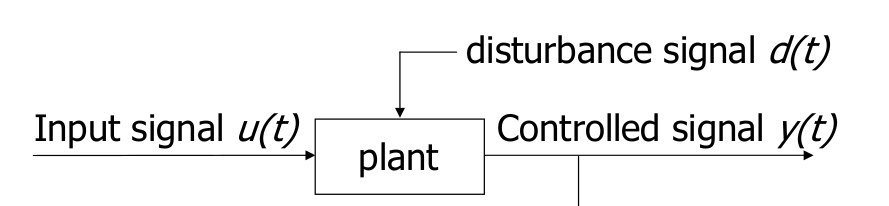
\includegraphics[scale=0.3]{noise.png}
    \caption{Rumore sommato all'Uscita}
    \label{fig:noise}
\end{figure}

Applicando l'approccio open loop:
\begin{align*}
    y(t) & = d(t) + f(u(t)) = \\
         & = d(t) + f\left( f^{-1}(r(t)) \right) = \\
         & = d(t) + r(t)
\end{align*}

Si definisce l'errore di tracking:
\begin{align*}
    e(t) & \triangleq \text{ errore di traking} \\
    e(t) & \triangleq y(t) - r(t) = d(t)
\end{align*}
\end{example}

Lo schema open loop non \`e in grado di attenuare i \emph{disturbi}, fallendo nell'obbiettivo di inseguire il riferimento. Va bene nel momento in cui il problema \`e molto semplice ed i disturbi hanno valori molto piccolo, potendo essere considerati trascurabili.

\subsubsection{Problema dell'Approssimazione}\label{sec:problema-dell-approssimazione}
Cosa succede se la nostra descrizione matematica del sistema risulta essere un' approssimazione dell'effettivo comportamento del sistema?
\begin{example}{}{}
    Si consideri la \autoref{fig:c-generatore-resistore} e si ipotizzi di voler regolare la grandezza $v(t)$. Si supponga che il modello matematico utilizzato sia: $y(t) = \widetilde{R} \cdot u(t)$, dove in generale $R \neq \widetilde{R}$. \\
    Il costruttore ci fornisce i dati sul resistore:
    \[ R = \widetilde{R} \pm \Delta R \]
    Dove $\Delta R$ \`e l'incertezza sulla misura. \\
    Si trova che:
    \begin{align*}
        y(t) & = R \cdot u(t) = \\
             & = R \cdot \frac{1}{\widetilde{R}} \cdot r(t) = \\
             & = r(t) \pm  \frac{\Delta R}{\widetilde{R}} \cdot r(t)
    \end{align*}
    Errore di tracking:
    \[ | e(t) | = \left| \frac{\Delta R}{\widetilde{R}} \cdot r(t) \right| \]
\end{example}

\begin{definition}{Errore di tracking}{errore-di-tracking}
    \[ | e(t) | = |y(t) - r(t)| \]
\end{definition}

Il controllo ad anello aperto fallisce l'obbiettivo di inseguire il riferimento perch\'e non \`e in grado di attenuare gli effetti degli \emph{errori di modello}.

\subsection{Controllo ad Anello Chiuso}\label{sec:controllo-ad-anello-chiuso}
Si \`e visto come la schema ad \emph{anello aperto} (\ref{sec:controllo-ad-anello-aperto}) non sia utile a risolvere il problema dell'inseguimento. La soluzione a tale problema, cha permette di abbandonare questo schema molto \emph{naive}, sar\`a il \textbf{controllo ad anello chiuso}, che verr\`a implementato tramite la \textbf{retroazione negativa} (\textbf{negative feedback}). Esso si basa su tre conclusioni fondamentali.

\subsubsection{Prima conclusione Fondamentale}\label{sec:prima-conclusione-fondamentale}
Un sistema di controllo pu\`o attenuare l'effetto di eventuali disturbi esterni e/o errori di modello se e solo se \`e presente una \textbf{retroazione negativa}. \\
\emph{L' intuizione \`e}: per attenuare l'effetto di disturbi e errori di modello, \`e necessario misurare istante per istante l'uscita $y(t)$ e confrontarla con l'uscita desiderata $r(t)$, come si vede in \autoref{fig:retroazione-negativa} l'uscita dell'impianto viene portata al controllore del sistema.
\begin{figure}[H]
    \centering
    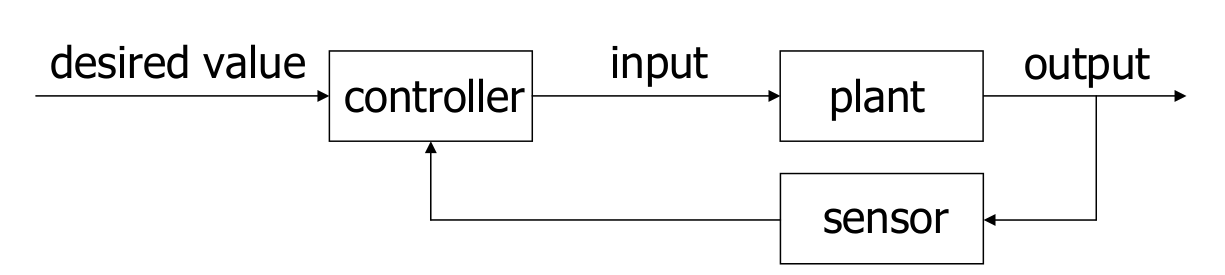
\includegraphics[scale=0.3]{retroazione-negativa.png}
    \caption{Retroazione Negativa}
    \label{fig:retroazione-negativa}
\end{figure}

Gli errori di modello e gli errori di disturbo sono i motivi per cui nasce la \emph{toria dei controlli automatici} e della \emph{teoria della retroazione negativa}.


\subsubsection{Seconda conclusione Fondamentale}\label{sec:seconda-conclusione-fondamentale}
Per controllare l'uscita di un sistema si ha bisogno di dei sensori che monitorino costantemenete il valore della uscita che si vuole controllare.


\subsubsection{Terza conclusione Fondamentale}\label{sec:terza-conclusione-fondamentale}
Progettare un sistema di controllo con retroazione per la \textbf{stabilizzazione di un sistema instabile}! \\
Il problema fu studiato per la prima volta nei laboratori \emph{Bell} durante i primi anni del '900, per cercare di risolvere il problema del rumore nello scambio di segnali, riuscendo a trovare come soluzione proprio l'uso della retroazione negativa, anche se in alcuni casi, partendo da un sistema stabile, con l'uso di certi tipi di segnali, il sistema diventava instabile. L'idea si svilupp\`o fino alla moderna teoria, grazie alla sforza di persone come \emph{Bode, Black, Nyquist,} ecc... \\
Grazie alla retroazione si pu\`o, ad esempio, risolvere il problema della \emph{levitazione magnetica}, che \`e un problema intrinsecamente instabile.


\subsubsection{Schema di Retroazione Generale}\label{sec:schema-di-retroazione-generale}
Uno schema di retroazione generale per un sistema ad anello chiuso \`e mostrato in \autoref{fig:schema-retroazione-generale}.
\begin{figure}[H]
    \centering
    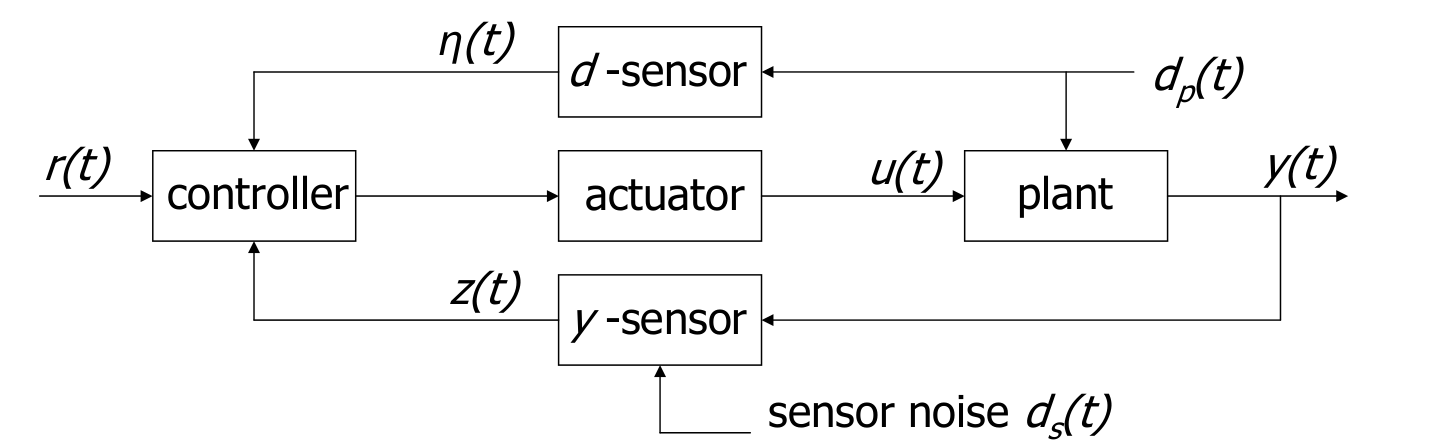
\includegraphics[scale=0.3]{schema-retroazione-generale.png}
    \caption{Schema di Retroazione Generale}
    \label{fig:schema-retroazione-generale}
\end{figure}

Il controllore che \`e il cervello del processo di automazione, attraverso i dati ricevuti dei sensori, da istruzioni al (o agli) attuatori. \\
Nella maggior parte dei casi i disturbi sono dei segnali non manipolabili e di solito non sono nemmeno misurabili. \`E possibile misurarli ($\eta$) solo in alcuni casi .


\newpage
\section{Sistemi Dinamici}\label{sec:sistemi-dinamici}
I sistemi si dividono in due tipologie: i sistemi statici ed i sistemi dinamici. \\
Nei sistemi statici la relazione tra ingresso ed uscita \`e univocamente determinata dell'ingresso a quel preciso istante $t_0$.
Un esempio di sistema statico \`e la relazione tra corrente $i(t)$ e la tensione $v(t)$ nella \autoref{fig:c-generatore-resistore}, infatti: $v(t) = Ri(t)$. \\
Un sistema \`e \textbf{dinamico} quando il valore dell'uscita dipende anche dai valori precedenti delle entrate e pi\`u in generale di tutta la storia passata del sistema.
Il modello maggiormente usato \`e quello dei sistemi dinamici, raramente dei modelli fisici possono essere rappresentati con dei sistemi statici.

\begin{example}{}{}
    Prendiamo come esempio un condensatore $C$ in serie con un generatore di corrente.
    \begin{figure}[H]
      \begin{center}
        \begin{circuitikz}
          \draw (0,0)
          to[I,i=$i(t)$] (0,2) % The voltage source
          to[short] (2,2)
          to[C,l_=$C$,v^<=$v(t)$] (2,0) % The resistor
          to[short] (0,0);
        \end{circuitikz}
      \end{center}
      \caption{Generatore di corrente con condesatore in parallelo}
      \label{fig:current-C}
    \end{figure}

    Secondo le relazioni fondamentali dell'elettrotecnica:
    \[ v(t) = \frac{Q(t)}{C} = \frac{1}{C} \cdot \int_{-\infty}^{t} i(t) dt \]
    \[ \Rightarrow y(t) = \frac{1}{C} \cdot \int_{-\infty}^t u(t) dt \]

    Il condesatore \`e un sistema dinamico in quanto l'uscita all'istante $t$ dipende da tutti i valori passati dell'ingresso fino a quell'istante $t$.
\end{example}

Come si pu\`o discrivere un sistema se la sua descrizione dipende da tutti gli stati pregressi? \\
Come si pu\`o ovviare al problema della necessit\`a di conoscere tutti i valori passati dell'ingresso?
\begin{align*}
    v(t) & = \frac{1}{C} \int_{-\infty}^t i(t)dt = \\
        \\
         & = \frac{1}{C} \left[ \int_{-\infty}^{t_0} i(t) dt + \int_{t_0}^t i(t) dt \right] = \\
        \\
         & = v(t_0) + \frac{1}{C} \int_{t_0}^t i(t) dt
\end{align*}

Non esiste il bisogno di conoscere tutta la storia passata del condensatore ma, basta conoscere la tesnione all'istante $t_0$, attraverso una misurazione delle sua carica totale. \\
% TODO: fornire un'esmpio
Per riuscire a descrivere l'uscita di un sistema si devono conoscere le \textbf{variabili di stato} (o \textbf{condizioni iniziali}) per poter descrivere la storia pregressa del sistema, queste variabili possono essere misurate. \\
Le variabili di stato possono essere trovate attraverso la risoluzione di \emph{equazioni differenziali}:
\begin{equation}\label{eq:condenser-relation}
    \frac{dv(t)}{dt} = \frac{1}{C} \cdot i(t)
\end{equation}
Per risolvere un'equazione differenziale si deve conoscere la \emph{forzante} ($u(t)$) e le \textbf{conidizioni iniziali} ($v(t_0)$). \\
Per descrivere un sistema in modo sistematico si applicano le leggi della fisica, la risultante del problema sono un insieme di equazioni differenziali che conterranno le variabili di stato.

\paragraph{\S Modellazione di un sistema}\label{par:modellazione-di-un-sistema}
Per modellare un sistema si individuano gli ingressi e le uscite. Gli ingressi possono essere di due titi:
\begin{itemize}
    \item manipolabili;
    \item non-manipolabili (disturbi);
\end{itemize}
Il numero di variabili di stato determinano l'ordine del sistema dinamico e sono sempre in numero fisso. \\
\`E possibile mostrare che \`e sempre possibile mostrare che \`e sempre possibile modellare un sistema fisico con una scelta di equazioni differenziali:
\begin{definition}{Equazioni di ingresso stato-uscita}{equazioni-di-ingresso-stato-uscita}
    (o \textbf{descrizione del sistema nella spazio dello stato}):
    \begin{equation}\label{eq:eq-ingresso-stato-uscita}
        \left\{
            \begin{array}{ll}
                \dot{\vv{x}}(t) = \vv{f}(\vv{x}(t), \vv{u}(t)) & \\
                \vv{y}(t) = \vv{g}(\vv{x}(t), \vv{u}(t)) & \\
            \end{array}
    \right. \quad\quad \forall t \begin{array}{ll}
            \vv{x} \in \mathbb{R}^n & \\
            \vv{u} \in \mathbb{R}^p & \\
            \vv{y} \in \mathbb{R}^q & \\
        \end{array}
    \end{equation}
\end{definition}
\begin{align*}
    \left\{ \begin{array}{ll}
            \dot{x_1}(t) = f_1(\vv{x}(t), \vv{u}(t)) & \\
            \dot{x_2}(t) = f_2(\vv{x}(t), \vv{u}(t)) & \\
            \quad\vdots & \\
            \dot{x_n}(t) = f_n(\vv{x}(t), \vv{u}(t)) & \\
        \end{array}
        \right. \quad\quad\quad \left\{ \begin{array}{ll}
            \dot{y_1}(t) = g_1(\vv{x}(t), \vv{u}(t)) & \\
            \dot{y_2}(t) = g_2(\vv{x}(t), \vv{u}(t)) & \\
            \quad\vdots & \\
            \dot{y_q}(t) = g_q(\vv{x}(t), \vv{u}(t)) & \\
        \end{array}
    \right.
\end{align*}

\begin{example}{Circuito RLC}{circuito-rlc}
    \begin{figure}[H]
        \centering
        \begin{circuitikz}
            \draw (0, 0)
            to [V=$v$,i=$i$] (0, 2)
            to [short] (1, 2)
            to [R,l_=$R$,v^=$v_R$] (3, 2)
            to [L,l_=$L$,v^=$v_L$] (5, 2)
            to [C,l_=$C$,v^=$v_C$] (5, 0)
            to [short] (0, 0);
        \end{circuitikz}
    \end{figure}
    Come primo punto si individua l'uscita e l'ingresso (scelte da noi):
    \begin{itemize}
        \item $y(t) = v_C(t)$
        \item $u(t) = v(t)$
    \end{itemize}
    Per trovare la \textbf{variabili di stato} di deve prima trovare l'equazione del sistema. \\
    Studio del sistema:
    \begin{itemize}
        \item $v_R = R i$
        \item $\frac{dv_C}{dt} = \frac{1}{C} i$
        \item $\frac{di}{dt} = \frac{1}{L} v_L$
        \item $ \vv{x}(t) = \begin{bmatrix} x_1(t) \\ x_2(t) \end{bmatrix} = \begin{bmatrix} i(t) \\ v_c(t) \end{bmatrix} $
    \end{itemize} Scelgo delle variabili di stato. Per dei sistemi elettronici le scelta che si pu\`o fare per prenere le variabili di stato sono: la tensione ai capi dei condensatori; le passanti per gli induttori. \\
    Si conosce da subito il grado del sistema (elettrico).
    \[ \frac{dx_1}{dt} = \frac{1}{L} \cdot v_L \]
    $v_L$ non \`e una variabile di stato, n\`e un ingresso, si devono trasformazioni per ricavarle.
    \[ KVL:\quad v_L = v - v_R - v_C \]
    \[ \dot{x_1} = -\frac{R}{L}x_1 - \frac{1}{L}x_2 + \frac{1}{L}u \]
    Calcoliamo $\dot{x_2}$:
    \[ \dot{x_2} = \frac{1}{C} \cdot i \]
    \[ \dot{x_2} = \frac{1}{C} \cdot x_1 \]
    \[ \Rightarrow \left\{ \begin{array}{l}
            \dot{x_1} = -\frac{R}{L}x_1 - \frac{1}{L}x_2 + \frac{1}{L}u \\
            \dot{x_2} = \frac{1}{C} x_1 \\
    \end{array} \right. \]
    Mentre $y(t)$:
    \[ y = x_2 \]
\end{example}

In generale le funzioni di stato e di uscita possono anche dipendere dal tempo (e.g. $g(t,x(t),u(t))$). Se questo \`e vero il sistema veiene definito \textbf{tempo-variante}. Se ci\`o non avviene il sistema viene detta \textbf{tempo-invariante}.

\paragraph{Tempo variante VS tempo invariante}
\begin{example}{}{}
    Circuito R.
    \begin{figure}[H]
        \centering
        \begin{circuitikz}
            \draw (0, 0)
            to [I=$i(t)$] (0, 2)
            to [short] (2, 2)
            to [R,v=$v_R$] (2, 0)
            to [short] (0, 0);
        \end{circuitikz}
    \end{figure}
    Sistema di ordine $0$ (sistema statico).
    \[ y = g(u) = R \cdot u \]
    \begin{itemize}
        \item[\boxed{C1}:] $R$ \`e un \emph{termistore} $\equiv$ il valore della sua resistenza dipende dalla sua temperatura.
            \[ y(t) = R(t)u(t) \;\to y(t) = g(t,u(t)) \]
            Sistema tempo-variante.
        \item[\boxed{C2}:] $R \equiv$ costante.
            \[ y(t) = Ru(t) \;\to y(t) = g(u(t)) \]
            Sistema tempo-invariante.
    \end{itemize}
\end{example}

\emph{OSS:} Se l'uscita del sistema dipende solo dalle variabili di stato ($u(t)$) \`e detto \textbf{strettamente proprio} $\to g(x(t))$.

\begin{example}{Single link manipulator}{single link manipulator}
    Si vuole controllare il momento di inerzia di un pendolo semplice, con le seguenti variabili:
    \begin{itemize}
        \item $\theta$ = angular position (variable of interest)
        \item m = mass
        \item l = link length
        \item $\beta$ = hinge friction coefficient
        \item u = applied torque at the hinge 
        \item g = gravity acceleration
    \end{itemize}

    Si usa l'equazione di Newton, con $J$ momento di inerzia, $M$ momento di una forza:
    \[ J \cdot \ddot{\theta} = \sum_i M_i \]

    Si scrivono le equazioni:
    \[ ml^2 \ddot{\theta}(t) = -mlg\sin(\theta(t)) - \beta \dot{\theta}(t) + u(t) \]
    \[ \Rightarrow \ddot{\theta}(t) = -\frac{g}{l} \sin(\theta(t)) - \frac{\beta}{ml^2}\dot{\theta}(t) + \frac{1}{ml^2}u(t) \]
    
    Per ovviare al problema delle derivate seconde si usa un trucco per le variabili di stato:
    \[ \vv{x}(t) = \begin{bmatrix} x_1 \\ x_2 \end{bmatrix} = \begin{bmatrix} \theta(t) \\ \dot{\theta}(t) \end{bmatrix} \]
\end{example}

\subsection{Sistemi Lineari Tempo-Invarianti}
Mettendo insieme la nozione di sistemi lineari e di tempo-invarianza si ottiene:
\[ \begin{system} \dot{x}(t) = Ax(t) + Bu() \\ y(t) = Cx(t) + Du(t) \end{system} \]
Dove in generale le matrici sono:
\[ A \in \RR^{n\times n}\quad B \in \RR^{n\times p}\quad C \in \RR^{q\times n}\quad \RR^{q\times p} \]

Si patr\`a sfruttare questo modollo anche per sistemi che non sono lineari. Questo modello non limita l'obbiettivo di progettare un sistema di controllo, nell'imporre un determinato comportamento chiediamo al sistema di inseguire le nostre uscite desiderate, anche in presenza di disturbi. L'obbiettivo \`e prendere un sistema ed imporre un certo comportamento. Si possono approssimare le equazioni non-lineari nell'intervallo di funzionamento a delle equazioni lineari.

Si user\`a  matlab (matrix laboratory) per descrivere questi modelli. Matlab semplificher\`a i calcoli attraverso operazioni tra matrici e vettori.

Per definire un vettore o una matrice la etichetto con un nome. Per definire una matrice si uano volori separati da spazi o da virgole, per gli elementi di una riga, si unano i punti e vergola. Per trasparre un matrice si usa un apice.

\begin{definition}{Polinomio Caratteristico}{polinomio-caratteristico}
    \[ det(\vv{A}-\lambda \vv{I}) \]
    Dove $\vv{I}$ \`e la matrice identit\`a.
\end{definition}
Ad esempio nelle matrici $3\times 3$ il polinomio caratteristico \`e:
\[ \lambda^3 + \alpha_2\lambda^2 + \alpha_1\lambda + \alpha_3 \]
\begin{definition}{Autovalore}{autovalore}
    Diciamo che $\lambda_i \in \RR$ \`e un autovalore delle matrice $\vv{A} \in \RR^{n\times n}$ se e solo se esiste un vettore $\vv{x}_i \in \RR^n$ (chimato autovettore corrispondente a $\lambda_i$) tale che:
    \[ \vv{A}\cdot  \vv{x}_i = \lambda_i \cdot \vv{x}_i \]
\end{definition}

Per colcolare gli autovalori su matlab si usa il comando \emph{eig()}.

\begin{definition}{Rango di una matrice}{rango-di-una-matrice}
    Il rango di una matrice \`e il numero di colonne o righe linearmente indipendenti.
\end{definition}
Per colcolare il ragno si usa \emph{rank()}.

Si suppinga di voler risolvere un sisetma lineare di equazione algebrciche:
\[ \vv{A}\cdot \vv{x} = \vv{b} \]
$\to \exists$ un'unica soluzione se e solo se (Hp: $A$ quadrata) $detA \neq 0 \Rightarrow \exists A^{-1} \Rightarrow \boxed{x = A^{-1}\cdot b}$.

Su matlab:
\begin{itemize}
    \item Se $A$ \`e invertibile $\Rightarrow \boxed{x = A\backslash b\triangleq A^{-1}\cdot b}$.
    \item Se $A \in R^{m\times n} (m > n) \Rightarrow \nexists A^{-1}$. \\
        In questo caso $x=A\backslash b$ fornisce la soluzione ai mininimi quadrati del sistema di equazioni $Ax =b$. Questa soluzione \`e fatta da:
        \[ Ax = b \]
        \[A^TAx = A^Tb \]
        Adesso $A^TA$ \`e quadrata. Se $det(A^TA) \neq 0$ allora
        \[ \boxed{x = (A^TA)^{-1}\cdot A^T\cdot b} \]
        Dove $(A^TA)^{-1}\cdot A^T \equiv$ pseudoinversa di $A$.
\end{itemize}
Matlab gesitsce entrabi i casi, sia di matrice quadrata sia che non lo sia. \`E possibile mostrare che: $x_{LS} = arg\;\underset{x}{min}|| Ax-b ||_2 $.

Per creare un sistema stato-uscita si usa il comando \emph{ss}, passando le matrici A, B, C e D.

\subsection{Sulzioni di Sistemi LTI}
Per risolvere un sisitema di equazini differenziali \`e necessario conoscere la forzante e le condizioni iniziali delle variabili di stato. Il risultato sar\`a la $x(t)$ e dunque si otterr\`a la $y(t)$.

Per risolvere le equazioni differenziale lineari a coefficenti costanti, l a soluzione \`e data dalla \textbf{equazione di Lagrange}:
\[ x(t) = e^{At} x(0) + \int_0^t e^{A(t-\tau)}Bu(\tau)d\tau = x_{zi}(t) + x_{zs}(t) \]
$x_{zi}$: \textbf{zero-input response} (risposta libera dello stato)  e dipende solo dalle condizione inziali, non dipende dalla forzante. \\
$x_{zs}$: \textbf{zero-state response} (risposta forzata dello stato), dipende dalla forzante che si va ad applicare sul sistema, che sia controllabile o non-controllabile.

Da qusta formula si pu\`o trovare l'andamento dell'uscita, dove si trovano nouvamente due termini: uno indipendte dalla forzante, uno dipendente dalla forzante, dette relativmte \textbf{risposta libera dell'uscita} e \textbf{rispsta forzata dell'uscita}.

Il problema dell'approccio attraverso l'equazionne di Lagrange \`e che ad ogni segnale diverso in entrata al sistema, va ricalcolato il valore dell'integrale, ci\`o comporta un problema computazionale non banale, sorgono maggiori problemi anche nel caso in cui la fuznione non sia integrabile analiticamente. Si usa allora la \textbf{Trasformata di Laplace}.

\begin{definition}{Trasformata di Laplace}{trasformata-di-laplace}
    \[ F(s) = \mathcal{L} \left\{f(t)\right\} \triangleq \int_0^\infty f(t)e^{-st} dt,\quad s \in \mathbb{C} \]
\end{definition}

Propiet\`a della trasformata di Laplace:
\begin{enumerate}
    % TODO: finire
    \item {\bf Linearit\`a}
    \item {\bf ok}
\end{enumerate}

% TODO: cambiare in theorem
\begin{theorem}{Teorema del valore finale}{teorema-del-valore-finale}
    \[ \lim_{t \to \infty} f(t) = \lim_{s \to 0^+} sF(s) \]
    Vale se e solo se i limiti sono entrabi finiti.
\end{theorem}

\begin{theorem}{Teorema del valore iniziale}{teorema-del-valore-iniziale}
    \[ \lim_{t \to 0^+} f(t) = \lim_{s \to \infty} sF(s) \]
    Vale se e solo se i limiti sono entrabi finiti.
\end{theorem}

Usando le trasformate di Laplace si potranno trasformare equazioni differenziali in equazioni algebriche.
\[ \begin{system} 
    \dot{x} = Ax +Bu \\
    y = Cx+Du
\end{system} \]

\[ \overset{\LL}{\longrightarrow}\quad \begin{system} 
    sX(s) - x(0) = AX(s) + BU(s) \\
    Y(s) = CX(s) + DU(s)
\end{system} \]

\begin{align*}
    \to\quad sX(s) - AX(s) & = x(0) + BU(s) \\
    (sI - A) X(s) & = x(0) + BU(s) \\
\end{align*}

\[ \to\quad \begin{system}
    X(s) & = (sI-A)^{-1} x(0) + (sI-A)^{-1} BU(s) \\
    Y(s) & = C(sI-A)^{-1} x(0) + [C(sI-A)^{-1}B + D]U(s)
\end{system} \]
\[ \begin{system}
    X = X_{zi} + X_{zs} \\
    Y = Y_{zi} + Y_{zs}
\end{system} \]
Bisogna tornare nel dominio del tempo.

I segnali utilizzati sono definiti solo per $t>0$, tutti i segnali sono implicitamente moltiplicati per il gradino unitario $\varepsilon(t)$.

I segnali pi\`u utilizzati sono: i polinomi, la delta di Dirac, esponenziali, sinusoidi. Per questi segnali esistono delle tabelle con le relative trasformate.

Usando Laplace, si procede per step:
\begin{enumerate}
    \item Trovare $X$ e $Y$ in $s$;
    \item Usare l'espansione in fratti semplici di Heaviside (PFE);
    \item Trovare i residui;
    \item Ottenere $x$ e $y$ antitrasformando;
\end{enumerate}

\begin{example}{}{}
    \[ \dot{x} = \begin{bmatrix} -3 & 2 \\ -2 & -3 \end{bmatrix}x + \begin{bmatrix} 1 \\ 0 \end{bmatrix} u \]
    \[ y = \begin{bmatrix} 0 & 1 \end{bmatrix}x + u \]
    Sapendo che $u = \varepsilon$ e $\vv{x}(0) = \begin{bmatrix} 1 \\ 1 \end{bmatrix} $.
    \[ Y(s) = C(sI-A)^{-1}x(0) + [C(sI-A)^{-1}B + D]U \]
    Svolgendo tutti i conti si ottiene
    \[ Y = \frac{s^{2}+s-2}{s(s+3-2j)(s+3-2j}  \]
    \[ y(t) = 1.38e^{-3t}\cos(2t+0.58)-0.15 \]
\end{example}
Ogni qual volta c'\`e una coppia di radici coniugate, si pu\`o dimostrare che anche i residui sono coniugati:
\[ \frac{R}{s-\sigma_0 -j\omega_0}  + \frac{R^{*}}{s-\sigma_0 +j\omega_0}  \]
La $\LL^{-1}$ corrisponde a:
\begin{definition}{Antitrasformata di Radici Coniugate}{antitrasformata-di-radici-coniugate}
    \[ 2\|R\| e^{\sigma_0t} \cos(\omega_0t + \angle R) \]
\end{definition}


\subsection{Matlab}
Per risolver un sistema di equazioni in matlab \`e necessario introdurre la variabile $s$. Si pu\`o definire la variabile $s$ con il comando \texttt{s = tf('s')} (dove \texttt{tf()} vuol dire Transfer Function). Sar\'a interpretata da ora in avanti come la pulsazione complessa.

Per cacolare l'uscita $Y$ a partire dal sistema si usa: 
\[ \texttt{Y = minreal(zpk(C*inv(s*eye(2)-A)*(B*U+x0)))} \]

\begin{itemize}
    \item Comando \texttt{zpk()}: viene calcolata la fattorizzazione dei polinomi al numeratore e denominatore;
    \item Comando \texttt{minreal()}: forza le semplificazioni in \texttt{zpk()} fissando una tolleranza (e.g. \texttt{G = funzione; minreal(zpk(G), 1e-6);}) semplifica zeri e poli con una tolleranza di $10^{-6}$);
\end{itemize}

Si procede dunque con la scomposizione in fratti semplici: si usa il comando \texttt{residue()} per trovare la rapresentazione vettoriale del numratore e del denominatore.
\[ \texttt{[numY, denY] = tfdata(Y,'v');} \]

Per trovare i poli e gli zeri si usa il comando \texttt{residue()}.
\[ \texttt{[r, p, k] = residue(numY, denY);} \]
Dove \texttt{r} ed \texttt{p} sono zeri e poli, mentre \texttt{k} \`e la costante sommata. Nei sistemi fisicamente realizzabile \texttt{k} \`e sempre zero, se cos\`i non fosse antitrasformando apparirebbe una delta, quindi un coportamento impulsivo: non fisicamente realizzabile.

In \emph{simulink} settando i parametri in auto, quando si simula un sistema, matlab previene (il pi\`u delle volte) che le soluzione delle equazioni differenziali divergano. Nella sezione della configurazione si pu\`o scelgiere il max step size di integrazione, se \`e troppo grande si richia di far divergere la soluzione dell'equazione. In simulink si possono caricare delle condizioni iniziali andandole ad inserire dentro gli integratori, nella sezione \emph{initial condition}, in questo modo si potr\`a vedere la solamente la risposta forzata, mentre quello libera rimane zero.

Per salvare i dati di una simulazione effettuata si usa il comando:
\[ \texttt{save nome-del-file-in-cui-salvare variabile [variabile ...];} \] 

Per caricare le variabili si usa il comando \texttt{load}:
\[ \texttt{load nome-file;} \]

Per caricare il simulink nello script si usa il comando \texttt{sim()}, questo ci resitituir\`a i parametri del sistema vista dal blocco \texttt{To Workspace}, \`e comodo impostare il valore di ritorno con \texttt{Structure With Time}.


\subsection{Rappresentazione in Funzioni di Trasferimento}
I sistemi LTI possono essere rappresentati attraverso fdt. Definizione di fdt di un sistema LTI.
\begin{definition}{Funzione di Trasferimento}{fdt}
    \[ \text{fdt} \triangleq H(s) \triangleq \left. \frac{Y(s)}{U(s)} \right|_{x(0) = 0} = C(sI-A)^{-1}B + D \]
    La fuznione di trasferimento vale solo quando le condizioni iniziali sono nulle.
\end{definition}

Dato un sitema descritto mediante una fdt, possiamo ricavare le equazioni di ingresso stato-uscita? Questo \`e un problema mal posto, infatti la fdt mescola tra di loro le matrici. Scelte diverse di matrici, possono portare ad ottenere la stessa fdt. Questo problema \`e detto \textbf{problema delle realizzazione} e non ha una soluzione univoca. Per risolvere il problema si applica una scelta arbitraria che mi conduce ad una fra le tante soluzioni.


\subsection{Stabilit\`a Interna}
Un esempio di sistema stabile \`e banalmente un pendolo, facendolo partire da una posizione iniziale la sua uscita tende a fermarsi sul centro (in presenza di attriti). \\
Un esempio di sistema instabile \`e un'asta in equilibio, con cui uno stimolo piccolissmo porta l'asta a cadere: il coefficente angolare va a $\infty$.
Un sistema \`e stabile se, sottoponendolo a degli stimoli finiti o a delle condizioni iniziali finite, l'uscita rimane finita.

\begin{definition}{Stabilit\`a Interna}{stabilita-interna}
    Fa riferimtnto alla risposta libera dello stato. Un sistema LTI \`e internamente stabile quando la risposta libera dello stato rimane limita per ogni condizione iniziale $\vv{x}_0 \in \RR^{n}$ finita.
\end{definition}

\begin{definition}{Stabilit\`a Asintotica}{stabilita-asintotica}
     Se la rispota libera tende a 0 per $t \to \infty$ allora il sistema \`e asintoticamente stabile. Se la risposta libera tende a zero allora \`e impolicitamente continua per tutti gli t.
\end{definition}

\begin{definition}{Instabilit\`a Interna}{instabilita-interna}
    Se si trova una sola condizione iniziale per cui la risposta libera diverge, allora il sistema \`e internamente instabile.
\end{definition}


Gli unici sistemi di interesse sono quelli asintoticamente stabili.

Stabilit\`a interna di un sistema LTI. \\
Troviamo un modo sistematico di desrivere il sistema a partire dalle equazioni del sistema, quando questo \`e internamente stabile. Partiamo dalla (\ref{def:equazioni-di-ingresso-stato-uscita}), cosiderando le radici del denominatore come reali e con moltiplicit\`a $1$.
\[ \vv{x} _{zi}(t) = \LL^{-1} \left\{ \vv{x} _{zi}(s) \right\} = \LL^{-1} \left\{ (s\vv{I}-\vv{A})^{-1}\vv{x} _{zi}(0) \right\} \]
\[ = \LL^{-1} \left\{ \begin{bmatrix} X_1(s) \\ X_2(s) \\ \vdots \\ X_n(s) \end{bmatrix} \right\} = 
\LL^{-1} \left\{ \begin{bmatrix} \frac{N _{X_1}(s)}{D _{X_1}(s)} \\ \vdots \end{bmatrix}  \right\} \]

\[ x_1(t) = \LL^{-1} \left\{ \frac{N _{X_1}}{D _{X_2}}  \right\} = \LL^{-1} \left\{ \frac{R_1}{s-p_1} + \dots \right\}  \]
\[ x_1(t) = R_1e^{p_1t} + \dots + R_ne^{p_nt} \]

\[ \boxed{ x_1(t) \underset{t \to \infty}{\longrightarrow} 0 \iff p_1,p_2,\dots,p_n < 0} \]

\[ \left| x_1(t) \right| < M \in \RR? \implies p_1,...,p_n \leqslant 0, \exists \text{almeno un volre } i :p_i = 0 \]

\[ x_1(t) \underset{t \to \infty}{\longrightarrow} \pm \infty ? \implies \exists i: p_i > 0 \]

\[ X(s) = (sI-A)^{-1}x(0) = \frac{1}{det(sI-A)} adj(sI-A) \begin{bmatrix} x_1(0) \\ \vdots \\ x_n(0) \end{bmatrix}  \]
\[ X_i(s) = \frac{1}{det(sI-A)} \left[ a _{ij}(s) \right] \begin{bmatrix} x_1(0) \\ \vdots \\ x_n(0) \end{bmatrix}  \]
\[ X_1(s) = \frac{1}{det(sI-A)} \left[ a _{11}(s) \dots a _{1n}(s) \right] \begin{bmatrix} x_1(s) \\ \vdots \\ x_n(0) \end{bmatrix}  \]
\[ = \frac{a _{11}(s)x_1(0) +\dots + a _{1n}(s)x_n(0) }{det(sI-A)}  \]
Dove $det(sI-A) = P_c(A)$:
\[ \boxed{ \implies p_1,\dots,p_n \text{ sono gli autovalori della matrice A! }} \]


Se esistono dei $p_i$ complessi coniguati che appratengono a $\mathbb{C}$, il sistema \`e asinticamente stabile $\iff$ tutte le parti reali degli autovalori \`e negativa. Nella risposta libera si potranno avere dei termini del tipo:
\[ 2|R|e^{\sigma_0t}\cos(\omega_0t+\angle R) \]
Anche in questo caso con una parte reale negativa, il termine converge a $0$.

Analizziamo il caso in cui la molteplicit\`a sia maggiore di $1$.
Scomposizione in fratti semplici di Heaviside in presenza di readici del donominatore con molteplicit\`a $> 1$:
\[ H(s) =  \frac{N_H(s)}{D_H(s)} = \frac{N_H(s)}{\prod_{i=1}^{N} (s-p_i)^{n_i} }  \]
\[ H(s) = \frac{R _{1,1}}{s-p_1} + \dots + \frac{R _{1,n_1}}{(s-p_1)^{n_1}} + \]
\[ + \frac{R _{2,1}}{(s-p_2)} + \dots + \frac{R _{2,n_2}}{(s-p_2)^{n_2}} + \]
\[ \frac{R _{m,1}}{(s-p_m)} + \dots + \frac{R _{m,n}}{(s-p_m)^{n_m}} \]

\[ h(t) = R_{1,1}e^{p_1t} + R_{1,2}te^{p_1t} + \dots + R _{1,n_1}\frac{t^{n_1-1}}{(n_1-1)!}e^{p_1t} + \dots \]

\[ \boxed{ h(t) \underset{t \to \infty}{\longrightarrow} 0 \iff \forall i : \sigma_i < 0 } \]

\begin{definition}{Criteri di Stabilit\`a}{criteri-di-stabilita}
    \begin{enumerate}
        \item \textbf{Stabilit\`a asintotica:} \\
            Un sistema LTI \`e asintoticamente stabile $\iff$ tutti gli autovalori della matrice $\vv{A}$ hanno parte reale strettamente negativa: $\forall i: \Re\left\{ \lambda_i \right\} < 0$.
        \item \textbf{Stabilit\`a interna (semplice):} \\
            Un sistema LTI \`e internamente stabile $\iff$ tutti gli autovalori della matrice $\vv{A}$ hanno parte reale minore o uguale a zero e quelli con parte reale nulla compaiono tra le radici del polinomio minimo $q_a$ con molteplcit\`a 1.
        \item \textbf{Instabilit\`a interna:} \\
            Un sistema LTI \`e internamnete instabile $ \implies $ non soddisfa le condizioni del risultato 2.
    \end{enumerate}
\end{definition}

\newpage
\subsection{Stabilit\`a BIBO}
\begin{definition}{Stabilit\`a BIBO}{stabilita-bibo}
    (O stabilit\`a interna) \`e legata alla risposta forzata. Un sistema \`e BIBO se la riposta forzata dell'uscita rimane limitata a fronte di segnali in ingresso limitati.
    \[ \forall u_M \in (0, \infty),\quad \exists y_M \in (0, \infty): \]
    \[ |u(t)| \leqslant u_M,\;\forall t \geqslant 0 \implies |y(t)| \leqslant y_M,\;\forall t \geqslant 0 \]
\end{definition}

Per capire sotto quali condizioni rimane limitata:
\[ Y _{zs}(s) = H(s)U(s) \]
\[ y _{zs}(t) = \LL \left\{ H\cdot U \right\} \text{ rimane limitata } \forall u, |u(t)| \leqslant M < \infty \quad M \in \mathbb{R} \]
\[ Y(s)  = \frac{N_H(s)N_U(s)}{D_H(s)D_U(s)}  = \frac{N_Y(s)}{\prod_{i=0}^{N} (s-p_i^{H}) \prod_{i=1}^{a} (s-p_i^{U}) }  \]

Le radici di $D_Y(s)$ si chimano poli del sistema.
La radici di $N_Y(s)$ si chimono zeri del sistema.

\begin{enumerate}
    \item Ipotizzione che $p_1^{H},\dots,p_N^{H},p_1^{U},\dots,p_a^{U}$ sono tutti distinti.
        \[ \implies Y(s) = \frac{R_1^{H}}{s-p_1^{H}} + \dots +\]
        \[ \implies y _{zs} = \LL^{-1} \left\{ \frac{R_1^{H}}{s-p_1^{H}}  \right\} + \dots +   \]
        $ \left|  y _{zs}(t) \right| $ sia limitato $\forall t$, $\forall u(t)$ limitato. Siccome per definizione $u(t)$ \`e limitato $ \implies\LL^{-1} \left\{ \frac{R_1^{U}}{s-p_1^{U}}  \right\} + \dots + \left\{ \frac{R_N^{U}}{s-p_N^{U}}  \right\}$ sono limitati. 
        \[ \boxed{ \implies |y(t)| \text{ \`e limitata } \iff p_1^{H},\dots,p_N^{H} \text{ sono tutti a parte reale } \leqslant 0}.\] 
        \item Assumiamo che $H$ e $U$ \underline{non} abbiano poli in comune.
        \[ Y _{zs}(s) = \frac{R_1^{H}}{(s-p_1^{H})} +\dots+ \frac{R_N^{H}}{(s-p_N^{H})} + \frac{R_1^{U}}{(s-p_1^{U})} +\dots + \frac{R_a^{U}}{(s-p_a^{U})} \]
        \[ y _{zs}(t) = \LL^{-1} \left\{ \frac{R_1^{H}}{(s-p_1^{H})} +\dots+ \frac{R_N^{H}}{(s-p_N^{H})}   \right\} +\LL^{-1} \left\{ \frac{R_1^{U}}{(s-p_1^{U})} +\dots+ \frac{R_a^{U}}{(s-p_a^{U})}  \right\}  \]
        Sotto quali ipotesi \`e limitata questa condizione ($u$ \`e limitata per ipotesi)?
        $\implies |y _{zs}|$ \`e limtata si solo se $p_1^{H},\dots,p_N^{H}$ sono tutti a parte reale $ \leqslant 0$ e i poli a parte reale nulla hanno molteplcit\`a para a 1.

    \item Nessuna assuznione sui poli di $H$ e $U$ $ \implies$ sto ammettendo la possibilit\`a che $D_H$ e $D_U$ abbiano radici in comune.

        Siccome $ |u(t)| \leqslant M < \infty \implies p_1^{U}(s),\dots,p_N^{U}(s) $ sono tutti a parte reale negativa o nulla.

        Le radici di $D_H$ eventualmente in comune con $D_U$ saranno a parte reale $ \leqslant 0$. 
        \begin{itemize}
            \item Ci sono radici in comune a parte reale $ < 0$: \\
                $ \implies D_Y$ avr\`a radici reali multiple a parte real $< 0 \implies$ modi asinticamente convergenti a 0.

            \item Ci sono radici in comune con parte reale nulla. \\
                $ \implies D_Y$ avr\`a radici con parte reale nulla e con molteplcit\`a $> 1 \implies$ \textbf{modi divergenti}.
        \end{itemize}

    \item BIBO stabilit\`a: \\
        Un sistema LTI \`e BIBO stabile $ \iff$ i poli della sua funzione di trasferiento $H(s) = C(sI-A)^{-1}B + D$ sono tutti a parte reale $< 0$.
\end{enumerate}

\subsection{Relazione tra Stabilit\`a Interna e BIBO}
$ x _{zi}(t) = \LL^{-1} \left\{ (sI-A)^{-1}x(0) \right\} : y _{zs}(t) = \LL^{-1} \left\{ [C(sI-A)^{-1}B + D] U(s) \right\} $
\[ \LL^{-1} \left\{ \frac{1}{det(sI-A)} [\dots]x(0) \right\}: \LL^{-1} \left\{ \left[  C\frac{1}{det(sI-A)}[\dots] B + D\right] U(s) \right\}  \]
Confrontando $X _{zi}$ e $Y _{zs}$ si pu\`o dedurre che i poli di $H$ sono un sottoinsieme (al pi\`u completo) degli autovalori della matrice $\vv{A}$.

Risultato 5: Se un sistema LTI $S$ \`e stabili \`e asinticamente stabile $ \implies$ $S$ \`e BIBO stabile.

Risultato 6: Se $S$ \`e BIBO instabile $ \implies$ $S$ non \`e asintoticamente stabile.


--

Per calcolare il polinomio minimo si deve trovare il mcm di tutti i den della matrice $\vv{A}$.
% TODO:  <25-03-22, da mettere sopra> %


Posso trovare la variabile $\tau$ che corrisponde all'intersizione dell'asse con la retta tangente in 0 dell'esponenziale.
\[ f(t) = e^{-\alpha t} \]
\[ \implies \tau = \frac{1}{\alpha}  \]

Per definire i tempi delle risposte forzate (vista la presenza degli esponenziali) si usa un metodologia:
\begin{verbatim}
    time = [0:tau/10:10*tau];
\end{verbatim}

Il motivo \`e che dope 5-volte $\tau$ l'esponenziale raggiunge il $99\%$ del suo valore finale, diventando trascurabile.


\section{Analisi in Regime Stazionario}
Si consideri un sistema asintoticamente stabile e BIBO stabile, allora la sua funzione di trasferimento \`e ha $n_h$ distinti poli $p_i$ con molteplicit\`a $\mu_i$, con $\Re[p_1] < 0, \;\forall i$.

Possiamo studiare la risposta forzata con un entrata $u(t)$ con trasformata di Laplace:
\[ U(s) = \frac{N_U(s)}{\prod_{j=1}^{n_u} (s-q_j)^{m_j} }  \]

Si ha un uscita:
\[ Y(s) = H(s)U(s) = \frac{N_H(s)}{\prod_{i=1}^{n_h} (s-p_i)^{\mu_i} } \cdot \frac{N_U(s)}{\prod_{j=1}^{n_u} (s-q_j)^{m_j} }   \]
\[ Y(s) = \sum_{i=1}^{n_h} \sum_{k=1}^{\mu_j} \frac{R _{i,k}}{(s-p_i)^{k}} + \sum_{j=1}^{n_u} \sum_{k=1}^{m_j} \frac{Q _{j,k}}{(s-q_j)^{k}}  \]

Si ottengono dunque due termini:
\begin{itemize}
    \item La \textbf{Risposta transitoria} ($y _{tr}(t)$): che tende a zero per t che tende all'infinito, questo \`e dato dal fatto che il sistema \`e BIBO stabile $ \implies$ $\Re[p_j] < 0, \;\forall i$.
    \item La \textbf{Risposta in regime stazionario} ($y _{ss}(t)$): che dipende solo dal segnale in entrata al sistema.
\end{itemize}

Si ottiene allora che:
\[ y(t) \underset{t \to \infty}{\longrightarrow} y _{ss}(t) \]

Posso definire queste riposte $ \iff$ il sistema \`e BIBO stabile o se le condizioni iniziali non sono nulle il sistema deve essere asintoticamente stabile.


% TODO:  <29-03-22, fire> %


Per trovare il valore delle risposta forzata si pu\`o usare il teorema del valore finale (\ref{the:teorema-del-valore-finale}). Il valore di $H(0)$ viene detto \textbf{guadagno in continua} (DC Gain). Su matlab si pu\`o usare il comando \texttt{dcgain();} per trovare il guadagno di una funzione di trasferimento.

\begin{definition}{Guadagno Stazionario Generalizzato}{guadagno-stazionario-generalizzato}
    \[ \lim_{s \to 0} s^{r}H(s) = K \]
\end{definition}

\subsection{Propriet\`a dello Stato Stazionario}
La risposta stazionaria al gradino $\bar{u}\varepsilon(t)$ \`e data da:
\begin{theorem}{Risposta al Gradino}{risposta-al-gradino}
    \[ u(t) = \bar{u}\varepsilon(t) \]
    \[ y _{ss}(t) = \bar{u}\cdot H(0) \]
\end{theorem}

Se un segnale in entrata ad un sitema BIBO stabile \`e sinusoidale, allora, anche la risposta stazionaria \`e sinusoidale.
\begin{theorem}{Risposta alla Sinusoide}{risposta-alla-sinusoide}
    \[ u(t) = \bar{u}\sin(\varphi t) \]
    \[ y _{ss}(t) = \bar{u}|H(\varphi)| \sin(\varphi t + \angle H(\varphi)) \]
\end{theorem}


\section{Sistemi Non-Lineari}
Un sitema dinamico non-lineare che ha uno stato costante $\bar{\vv{x}}$ \`e una \textbf{soluzione di equilibrio} se, nella presenza di un input costane $\vv{u}(t) = \bar{\vv{u}}$ e delle condizioni iniziali $\vv{x}(0) = \bar{\vv{x}}$, risulta:
\[ \vv{x}(t) = \bar{\vv{x}}, \;\forall t \geqslant 0 \]

Allora:
\begin{itemize}
    \item $\bar{\vv{u}}$: ingresso di equilibrio;
    \item $(\bar{\vv{x}},\bar{\vv{u}})$: punto di equilibrio;
    \item $\vv{g}(\bar{\vv{x}},\bar{\vv{u}})$: uscita di equilibrio;
\end{itemize}

Un punto di equilibrio soddifa la condizione di equilibrio:
\[ \vv{f}(\bar{\vv{x}},\bar{\vv{u}}) = \vv{0} \]

\begin{example}{Levitazione Magnetica}{levitazione-magnetica}
    % TODO:  <31-03-22 finire quando ho finto tutta la prarte sulla linearizzazione> %
    \begin{figure}[H]
        \centering
        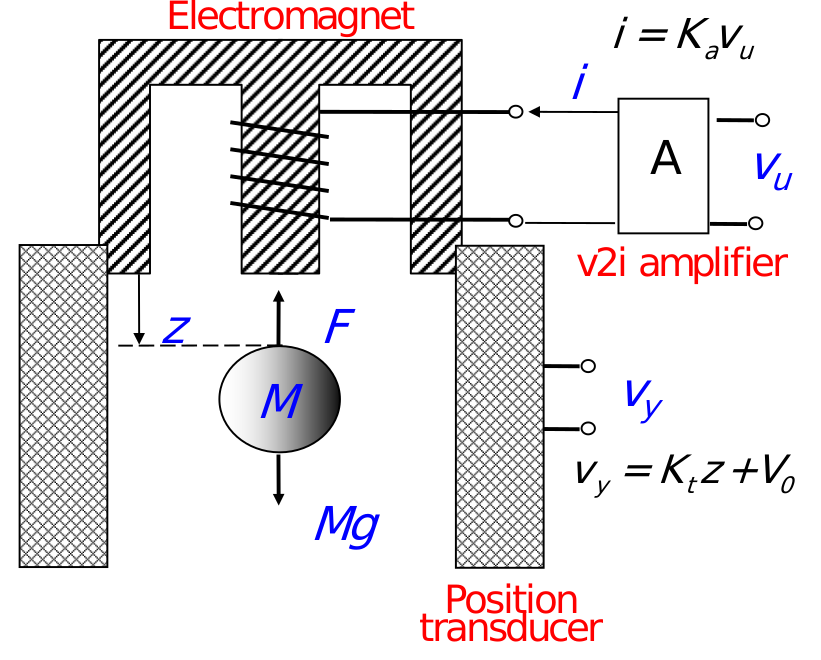
\includegraphics[width=0.5\textwidth]{levitazione-magnetica.png}
        \caption{Levitazione Magnetica}
        \label{fig:levitazione-magnetica}
    \end{figure}

    \[ M\ddot{z} = Mg - F \]
    \[ F = \frac{B_m i^{2}}{z^{2}}  \]

    Rappresentazione stato-uscita:
    \[ x = \begin{bmatrix} z \\ \dot{z} \end{bmatrix}  \]
    \[ u = v_u(t) \]
    \begin{align*}
        & \begin{system} \dot{x}_1 = x_2 \\
        \dot{x}_2 = g\end{system} 
    \end{align*}

\end{example}

\subsection{Linearizzazione di Sistemi Non-Lineari}
I sistemi nel mondo reale sono, in generale, non-lineari. Per studiarli si pu\`o approssimare il comportamento in un intorno di una soluzione (come soluzione di equilibrio) attraverso dei sistemi modelli linari detti \textbf{modelli linearizzati}.

Per approssimare il modello si usa uno sviluppo in serie di Taylor troncato al primo membro, in questo modo il sistema risultate sar\`a lineare.
\[ \vv{f}(\vv{x}) = \vv{f}( \vv{x}_0 + \delta\vv{x}) \]
\[ = \vv{f}(\vv{x}_0) + \frac{d \vv{f}}{d \vv{x}}(\vv{x}_0) \cdot (\vv{x} - \vv{x}_0) \]
\[  = \vv{f}(\vv{x}_0) + \frac{d \vv{f}}{d \vv{x}}(\vv{x}_0) \cdot \delta\vv{x}  \]

Dove:
\[ \frac{d \vv{f}}{d \vv{x}}(\vv{x})  = \begin{bmatrix} 
    \nabla^T f_1(\vv{x}) \\
    \vdots \\
    \nabla^T f_n(\vv{x}) 
\end{bmatrix} =
\begin{bmatrix} 
        \frac{\partial f_1}{\partial x_1} & \dots & \frac{\partial f_1}{\partial x_m}  \\
        \vdots & \ddots & \vdots \\
        \frac{\partial f_n}{\partial x_1} & \dots & \frac{\partial f_n}{\partial x_m} 
\end{bmatrix} \]

\begin{definition}{Matrice Jacobiana}{matrice-jacobiana}
    Sia: $\vv{f}: \RR^m \to \RR^n$
    \[ \vv{J}\vv{f}(\vv{x}) \triangleq \begin{bmatrix} 
        \frac{\partial f_1}{\partial x_1} & \dots & \frac{\partial f_1}{\partial x_m}  \\
        \vdots & \ddots & \vdots \\
        \frac{\partial f_n}{\partial x_1} & \dots & \frac{\partial f_n}{\partial x_m} 
    \end{bmatrix}  \]
\end{definition}

Applicando piccole variazioni ai valori delle entrate e degli stati del sistema dello spazio delgi stati, dove $(\bar{\vv{x}}, \bar{\vv{u}}) = \vv{Q}$ \`e un punto di equilibrio del sistema, si ottiene:
\[ \begin{system} 
    \dot{\vv{x}} = \vv{f}(\vv{x},\vv{u}) \\
    \vv{u}(t) = \bar{\vv{u}} + \delta\vv{u}(t) \\
    \vv{x}(0) = \bar{\vv{x}} + \delta\vv{x}(t) 
\end{system}  \]

Risolvere un problema di Cauchy non-lineare non \`e facile, allora si linearizza il sistema, come primo passo si esprime la variazione della derivata dello stato come:
\[ \delta\dot{\vv{x}} = \dot{\vv{x}} - \dot{\bar{\vv{x}}} = \vv{f}(\vv{x},\vv{u}) + \vv{0} = \vv{f}(\vv{x},\vv{u})  \]

Si supponga che $\vv{f}$ abbia espansione di Taylor in un intorno di $\vv{Q}$, allora la sue espressione diventa:
\begin{align*}
    \vv{f}(\vv{x},\vv{u}) & = \vv{f}(\bar{\vv{x}}+\delta\vv{x}, \bar{\vv{u}}+\delta\vv{u}) = \\
                          & = \vv{f}(\vv{Q}) + \frac{\partial \vv{f}}{\partial \vv{x}} (\vv{Q}) \cdot (\vv{x}-\bar{\vv{x}}) +
                          \frac{\partial \vv{f}}{\partial \vv{u}} (\vv{Q}) \cdot (\vv{u} - \bar{\vv{u}}) \\
                          & = \boxed{ \vv{J}_{\vv{x}} \vv{f} (\vv{Q}) \cdot \delta\vv{x} + \vv{J}_\vv{u}\vv{f}(\vv{Q})\cdot \delta\vv{u} }
\end{align*}

Dove $\vv{f}(\vv{Q}) = \vv{0}$, essendo $\vv{Q}$ un punto di equilibrio del sistema. \\
Vale allora le seguente eguaglianza:
\[ \boxed{ \delta\dot{\vv{x}} =  \vv{J}_{\vv{x}} \vv{f} (\vv{Q}) \cdot \delta\vv{x} + \vv{J}_\vv{u}\vv{f}(\vv{Q})\cdot \delta\vv{u}  } \]

Si pu\`o effettuare un ragionamento simile per la variazione dell'uscita:
\[ \boxed{ \delta\vv{y} =  \vv{J}_{\vv{x}} \vv{g} (\vv{Q}) \cdot \delta\vv{x} + \vv{J}_\vv{u}\vv{g}(\vv{Q})\cdot \delta\vv{u}  } \]

\begin{definition}{Matrici Delle Variazioni}{matrici-delle-variazioni}
    \begin{flalign*}
       & \quad\bullet\quad \vv{A} = \vv{J}_\vv{x} \vv{f}(\vv{Q}) \in \RR^{n \times n} & \\
       & \quad\bullet\quad \vv{B} = \vv{J}_\vv{u} \vv{f}(\vv{Q}) \in \RR^{n \times p} & \\
       & \quad\bullet\quad \vv{C} = \vv{J}_\vv{x} \vv{g}(\vv{Q}) \in \RR^{q \times n} & \\
       & \quad\bullet\quad \vv{D} = \vv{J}_\vv{u} \vv{g}(\vv{Q}) \in \RR^{q \times p} & 
   \end{flalign*} 
\end{definition}

Si ottiene un sistema lineare della forma:
\begin{definition}{Sistema Linearizzato}{sistema-linearizzato}
    \[ \begin{system} 
    \delta \dot{\vv{x}} = \vv{A}\delta\vv{x} + \vv{B}\delta\vv{u} \\
    \delta\vv{y} = \vv{C}\delta\vv{x} + \vv{D}\delta\vv{u}
    \end{system}  \]
\end{definition}


\subsection{Stabilit\`a di Equilibrio}
Intuitivamnte parlando, un punto di equilibrio si dice \textbf{stabile} si tutte le soluzioni in un intorno di $\bar{\vv{x}}$  rimangono nello stesso intorno $\forall t$.

Un punto di equilibrio $\bar{\vv{x}}$ \`e detto \textbf{asintoticamente stabile} se \`e stabile e, tutte le soluzioni in un intorno di $\bar{\vv{x}}$ tendono a $\bar{\vv{x}}$ per $t \to \infty$.

Se la suluzione in un introrno dell'equilibrio diverge al di fouri dell'intorno il punto \`e \textbf{instabile}.

Un pendolo ha un punto di equilibrio stabile quando \`e appeso verso il basso mentre, ha un punto di equilibrio instabile quando \`e punta verso l'alto. Se il pendolo \`e smorzato il punto di equilibrio stabile diventa un punto di equilibrio asintoticamente stabile.

Per studiare un soluzione in equilibrio $\vv{Q}$ di un sitema dinamico si introduce una variazione della soluzione $\vv{x}_p(t)$, ottenuta in presenza di:
\begin{itemize}
    \item Lo stesso ingresso di equilibrio $\bar{\vv{u}}$;
    \item Un opportuno stato iniziale $\vv{x}_0$ in un intorno di $\bar{\vv{x}}$;
\end{itemize}

\begin{definition}{Stabilit\`a Dell'Equilibrio}{stabilita-dellequilibrio}
    La stato $\bar{\vv{x}}$ \`e stabile se:
    \[ \forall \varepsilon > 0, \;\exists \delta = \delta(\varepsilon) > 0: \]
    \[ \forall \vv{x}_0: \;\| \vv{x}_0 - \bar{\vv{x}} \| < \delta, \implies \| \vv{x}_p(t) - \bar{\vv{x}} \| < \varepsilon, \;\forall t\]
\end{definition}

\begin{definition}{Stabilit\`a Asintotica Dell'Equilibrio}{stabilita-asintotica-dellequilibrio}
    Lo stato $\bar{\vv{x}}$ \`e asintoticamente stabile se:
    \[ \lim_{t \to \infty} \| \vv{x}_p(t) - \bar{\vv{x}} \| = 0 \]
\end{definition}

Nel caso dei sistemi lineari:
\begin{itemize}
    \item \textbf{stabilit\`a interna} $\iff$ \textbf{stabilit\`a} di ogni punto di equilibrio;
    \item \textbf{stabilit\`a asintotica} $\iff$ \textbf{stabili\`a asitntotica} di ogni punto di equilibrio;
    \item \textbf{instabile} $\iff$ \textbf{instabilit\`a} di ogni punto di equilibrio;
\end{itemize}

Per i sisetmi LTI, la stabilit\`a interna \`e una propriet\`a globale che si applica ad ogni soluzione.


\subsection{Stabilit\`a di un Sisetema Linearizzato}
Per i sisetmi non-lineari, la stabili\`a \`e un concetto locale, legato all'intorno di una soluzione.

Dato un punto stabile $\vv{Q}$ di un sistema $\dot{\vv{x}} = \vv{f}(\vv{x}, \vv{u})$, dove $\vv{f}: D \to \RR^{n}, \;\vv{f}\in C^{1} $, dove $D$ \`e un intorno di $\bar{\vv{x}}$. Data:
\[ \vv{A} = \vv{J}_\vv{x}\vv{f}(\vv{Q}) \]

Allora, dati $\lambda_i(\vv{A})$ gli autovalori di $\vv{A}$:
\begin{itemize}
    \item $\forall i: \Re[\lambda_i(\vv{A})] < 0$ $ \implies$ asintoticamente satbile
    \item $\exists i: \Re[\lambda_i(\vv{A})] > 0$ $ \implies$ instabile
    \item $\forall i: \Re[\lambda_i(\vv{A})] \leqslant 0$ $ \implies$ non si possono trarre delle conclusioni
\end{itemize}



\newpage
\section{Risposta in Frequenza}
Data una funzione di trasferminto di un sistema lineare, si ottiene la \textbf{Risposta in Frequenza} sostituendo la variabiele $s\in \mathbb{C}$ con la variabile $j\omega, \omega\in\RR$.

\subsection{Diagrammi di Bode}
Per rappresentare la risposta in frequenza si usano i diagrammi di \textbf{Bode}. Si usa rappresentazione del tipo:
\[ H(s) = K \frac{\prod_{m=1} (1 - \frac{s}{z_m}) }{ s^{r} \cdot \prod_{n=1} (1- \frac{s}{p_n} )  }  \]
Data la \emph{f.d.t.}, si passa alla risposta in frequenza utilizzando $s = j\omega \implies H(j\omega)$:
\begin{itemize}
    \item $K$: (\textbf{guadagno in continua}) dB contributo cosatnte; non da contributo alla fase, se $K$ \`e negativo il contributo alla fase \`e di $-\pi = -180^{\circ}$;
    \item $\displaystyle \frac{1}{s} $: (\textbf{polo nell'origine}) dB contributo di $-20dB/dec$; fase contributo di $-\frac{\pi}{2}$;
    \item $s$: (\textbf{zero nell'origine}) dB contributo di $20dB/dec$; fase contributo di $\frac{\pi}{2} $;
    \item $\displaystyle \frac{1}{1-\frac{s}{p} } $: (\textbf{polo reale}) dB cotributo di $-20dB/dec$ in $p$; se il polo \`e negativo la fase ha un contributo di $-\frac{\pi}{2} = -90^{\circ}$, altrimenti (polo positivo) sale di $\frac{\pi}{2} $;
    \item $\displaystyle \left( 1- \frac{s}{z} \right)$: (\textbf{zero reale}) dB contributo di $20dB/dev$ in $z$; se lo zero \`e negativo la fase un contributo di $\frac{\pi}{2} = 90^{\circ}$, altrimenti di $-90^{\circ}$;

    \item $\displaystyle \frac{1}{\displaystyle 1+2 \frac{\zeta}{\omega_n}s + \frac{s^{2}}{\omega_n^{2}} }$: (\textbf{poli complessi coniugati})

        $\zeta$ viene detto smorzamento, ed \`e compreso tra $0 \leqslant \zeta \leqslant 1$. Compare un \textbf{picco di risonanza}, che diventa pi\`u alto per $\zeta$ che tende a 0. Nella frequnza $\omega_n$ c'\`e un contributo sul modulo di $-40dB/dec$. Se i poli sono complessi coniugati negativi, la fase ha un contibuto di $-180^{\circ}$, inoltre per $\zeta$ che tende a 0 la fase ha pendenza maggiore fino a diventre una retta verticale per $\zeta = 0$, se sono conigati positivi si ha un contributo di $180^{\circ}$
        \begin{figure}[H]
            \centering
            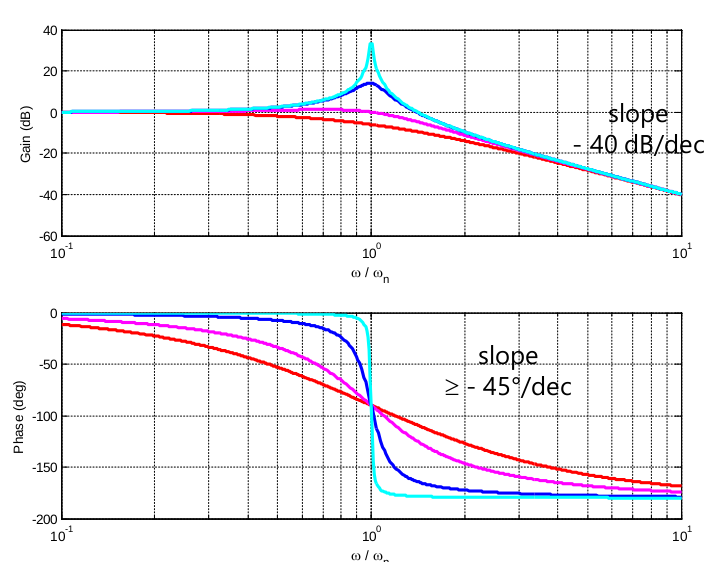
\includegraphics[width=0.5\textwidth]{effetto-smorzamento.png}
            \caption{Effetto Smorzamento}
            \label{fig:effetto-smorzamento}
        \end{figure}

        Nell'intorno di $\omega_n$ si trova questo picco, il cui valore massimo pu\`o essere espresso dalla formula:
        \[ M_r = \frac{1}{2\zeta \sqrt{1 - \zeta^{2}}}  \]

        alla frequenza:
        \[ \omega_r = \omega_n \sqrt{1 - 2\zeta^{2}} \]

    \item $\displaystyle 1 + 2 \frac{\xi}{\omega_n}s + \frac{s^{2}}{\omega_n^{2}} $: (\textbf{zeri complessi coniugati})

        Per gli zeri coniugati si ha un contriuto di $40dB/dec$ sul modulo; per zeri negativi si ha un contributo di $180^{\circ}$ sulla fase, mentre per zeri positivi si ha un contributo di $-180^{\circ}$.
\end{itemize}

\subsection{Diagrammi Polari}
Si pu\`o usare una rappresentazione polare, usando la parte immaginaria contro la parte immaginaria su un grafico $(\Re[H(j\omega)],\;\Im[H(j\omega)])$, variando la frequenza si ottiene una curva sul grafico.
% TODO:  <06-04-22, metter una fig> %

\subsection{Diagrammi di Nichols}
Il diagramma di Nichols \`e una rappresentazione della funzione di trasferimento plottata su un grafico con modulo della $H$ contro la fase della $H$, $(\angle H(s), |H(s)|)$.

Per creare un diagramma di nichols su matlab si usa:
\begin{lstlisting}
omega = logspace(x1, x2, N);
nichols(H, omega);
\end{lstlisting}
% TODO:  <06-04-22, mettere figura> %


\subsection{Diagramma di Nyquist}

\begin{definition}{Contorno di Nyquist}{contorno-di-nyquist}
    \`E una curva $\Gamma: \RR \to \mathbb{C}$, definita come:
    \[ \tilde{\Gamma}(\omega) = \Gamma_1(\omega) +  \Gamma_2(\omega) + \Gamma_3(\omega) \]
    \[ \Gamma_1(\omega) = jR\cdot\omega,\; \omega \in [0, 1] \]
    \[ \Gamma_2(\omega) = Re^{j\omega},\;\omega \in \left[\frac{\pi}{2}, -\frac{\pi}{2} \right]  \]
    \[ \Gamma_3(\omega) = jR\cdot(\omega-1),\; \omega \in [0, 1] \]
    \[\lim_{R \to \infty} \tilde{\Gamma} = \Gamma \]
\end{definition}

\begin{definition}{Diagramma di Nyquist}{diagramma-di-nyquist}
    Il diagramma di Nyquist $\Gamma_N$ \`e definito come l'immagine sul piano complesso $(\Re[H], \Im[H])$, della funzione $H(s)$ calcolata sul contorno di Nyquist.
    \[ \Gamma_N = (H \circ \Gamma) \]
\end{definition}

Nel caso in cui $H(s)$ ha poli a parte reale nulla, il diagramma di Nyquist va modificato, il motivo \`e che la funzione di trasferimento non pu\`o essere calcolata. Per ovviare a questo problema si possono posson inserire dei semicerchi di raggio infinitesimo in senso anti-orario, questo corrisponde sul diagramma di Nyquisti ad un semicerchio di raggio infinito e senso orario.

% TODO:  <06-04-22, mettere immagini> %



\section{Propriet\`a Strutturali}
L'analisi delle Raggiungilbilit\`a misura quanto l'ingresso riesce a modificare le variabili di stato.

\begin{definition}{Raggiungibilit\`a}{raggiungibilita}
    Uno stato $\vv{x}^{*} \in \RR^{n}$ ($\RR^{n}$: \textbf{spazio di stato}) si dice \textbf{raggiungibile} (dallo stato $\vv{x}_0$ al tempo $t^{*}$), se:
    \begin{itemize}
        \item $\exists$ un istante di tempo $t^{*} \in [t_0, \infty)$;
        \item $\exists$ una funzione di ingresso $\vv{u}^{*}(t)$ definita in $t \in [t_0, t^{*}]$;
    \end{itemize}
    tali che, il movimento della stato generato da $\vv{u}^{*}$ a partire dalla stato $\vv{x}_0$, risulti:
    \[ \boxed{\vv{x}(t^{*}) = \vv{x}^{*}} \]
\end{definition}

Nello spazio di stato posso definire tutti i punti che sono raggiungibili.
\begin{definition}{Insieme di Raggiungibilit\`a}{insieme-di-raggiungibilita}
    L'insieme di tutti i punti raggiungibili in $t^{*}$ \`e l'insieme:
    \[ X_R(t^{*}) \]
\end{definition}

Cambiando l'interallo di tempo l'insieme di raggiungibilit\`a, in generale, cambia. Si pu\`o trovare l'insieme di raggiungibilit\`a massimo.
\begin{definition}{Sottospazio di Raggiungibilit\`a}{sottospazio-di-raggiungibilita}
    \[ X_R = \underset{t\in[t,\infty)}{max} X_R(t^{*}) \]
\end{definition}

\begin{definition}{Sistema Completamente Raggiungibile}{sistema-completamente-raggiungibile}
    Se il sottospazio di raggiungibilit\`a coincide con lo spazio di stato \`e detto \textbf{completamente raggiungibile}.
    \[ X = X_R \]
\end{definition}

\begin{definition}{Sottospazio di Non-Raggiungibilit\`a}{sottospazio-di-non-raggiungibilita}
    \[ X _{NR} = X_R^{\perp} \]
\end{definition}

\begin{definition}{Stato Controllabile}{stato-controllabile}
    Partendo da stati iniziali nulli, si pu\`o raggiungere lo stato:
    \[ \vv{x}(t^{*}) = \vv{x}_0 \]
\end{definition}

Per la Controllabilit\`a valgono delle definizioni analoghe alla Raggiungibilit\`a.

\textbf{Per i sistemi LTI Tempo Continuo Controllabilit\`a e Raggiungibilit\`a coincidono:}
\[ \boxed{ X_R = X_C } \]

Un sistema con variabili di stato di dimensione $n$:
\begin{itemize}
    \item AL sottospazio di raggiungibilit\`a sono associati $r$ autovalori della matrice $\vv{A}$;
    \item Al sottospazio di non-raggiungibilit\`a sono associati $n-r$ autovalori della matrice $\vv{A}$;
    \item $dim(X_R) = r < n$;
    \item $dim(X _{NR}) = n-r$;
\end{itemize}

Se $r = n$ il sistema \`e completamente raggiangibile.


\subsection{Raggiungibilit\`a nei Sistemi LTI TD}
Prendiamo ora in esempio un sistema LTI a tempo discreto.
\begin{definition}{Sistema LTI TD}{sistema-lti-td}
    \[ \vv{x}(k+1) = \vv{Ax}(k) + \vv{Bu}(k), \;\forall k \in \mathbb{N} \]
\end{definition}

Troviamo il sottoinsieme di raggiungibilit\`a $X_R(l)$ al tempo $l$. Per semplicit\`a usiamo un sistma con un solo ingresso $u$ e con condizioni iniziale nulle.
\begin{align*}
    x(1) & = Ax(0) + Bu(0) = Bu(0) \\
    x(2) & = Ax(1) + Bu(1) = ABu(0) + Bu(1) \\
    x(3) & = Ax(2) + Bu(2) = A^{2}Bu(0) + ABu(1) + Bu(2) \\ 
         & \vdots \\
    x(l) & = A^{l-1}Bu(0) + \dots + ABu(l-2) + Bu(l-1)
\end{align*}

Si pu\`o usare una notazione matriciale per rappresentare $\vv{x}(l)$:
\begin{align*}
\vv{x}(l)  & = \underbrace{\begin{bmatrix} 
        B & AB & \dots & A^{l-1}B
        \end{bmatrix}}_{\vv{M}_R(l)} \underbrace{\begin{bmatrix} 
    u(l-1) \\
    u(l-2) \\
    \vdots \\
    u(0)
\end{bmatrix} }_{\vv{U}(l)} \\
    & = \vv{M}_R(l) \vv{U}(l)
\end{align*}

La matrice $\vv{M}_R(l) \in \RR^{n \times l}$ fornisce un legame diretto tra la sequenza di entrata e lo stato $x(l)$. L'insieme di raggiungibilit\`a $X_R(l)$ \`e dato dallo \textbf{spazio immagine} della matrice $\vv{M}_R(l)$:
\[ X_R(l) = \mathcal{R}\Bigl( M_R(l) \Bigr) \]

Per determinare il sottospazio di raggiungibilit\`a bisogna trovare l'insieme di raggiungibilit\`a massimo:
\[ X_R = \underset{t \in \RR^{+}}{\max}\, X_R(l) \]

La dimensione dell'insieme di raggiungibilit\`a corrisponde al rango della matrice $M_R$, che viene definta come \textbf{matrice di raggiungibilit\`a}.
\begin{definition}{Matrice di Raggiungibilit\`a}{matrice-di-raggiungibilita}
\[ M_R = \begin{bmatrix} B & AB & \dots & A^{n-1}B \end{bmatrix}  \]
\end{definition}

Il rango pu\`o aumentare al  massimo di uno per ongi colonna che viene aggiunta alla matrice, fino al raggiungere il massimo possibile che \`e $n$, dunque la dimensione dello spazio di raggiungibilit\`a \`e dato da:
\[ X_R = \rho (M_R) = r \]

Se $\rho(M_R) = n$ allora il sistema \`e completamente raggiungibile.

Questo risultato ottenuto per i sistemi a tempo discreto \`e generalizzabile anche ai sistemi a tempo continuo con un nunmero di ingressi maggiore di 1, dove:
\[ M_R = \begin{bmatrix} B & AB & \dots & A^{n-b}B \end{bmatrix}, \quad b = \rho(B) \]

\subsection{Matlab}
La matrice di raggiungibilit\`a pu\`o essere colcolata come:
\begin{lstlisting}[language=matlab]
M_R = ctrb(A, B);
r = rank(M_R);
\end{lstlisting}


\newpage
\section{Feedback}
\paragraph{\S~Schema di Controllo in Feedback}
Si usa uno schema di retroazione statica della stato, che si basa sul comportamento di un sistema LTI:
\begin{itemize}
    \item Il comportamento dinamico dipende dai valori della matrice $\vv{A}$;
    \item La possibilit\`a di modificare il suo comportamento dipende dalla raggiungibilit\`a, che dipende dalle matrici $\vv{A}$ e $\vv{B}$;
\end{itemize}
Agendo in retroazione si vuole:
\begin{itemize}
    \item rendere asintoticamente stabile un sistema instabile;
    \item migliorare le proprit\`a di movimento di un sistema stabile come: smorzamento, rapidit\`a di convergenza;
    \item portare la stato del stistema in uno stato di equilibrio;
\end{itemize}

\subsection{Legge di Controllo}
Per modificare il comportamento dinamico del sitema l'ingresso $u$, deve poter agire sugli stati $x$, questo pu\`o avvenire se $x$ dipende dallo stato in tale relazione:
\begin{definition}{Legge Di Controllo Per Retroazione Statica Dello Stato}{legge-di-controllo-per-retroazione-statica-dello-stato}
    \[ u(t) = -\vv{Kx}(t) + \alpha r(t) \]
\end{definition}

Dove:
\begin{itemize}
    \item $\vv{x}(t) \in \RR^{n}$;
    \item $u(t) \in \RR$;
    \item $\vv{K} \in \RR^{1 \times n}$: matrice dei guadagni;
    \item $r(t) \in \RR$: ingresso esterno;
    \item $\alpha \in \RR$;
\end{itemize}


Si pu\`o considerare lo schema:
\begin{figure}[H]
    \centering
    \begin{tikzpicture}[scale=0.4,auto, node distance=3cm]
        \node[coordinate] (input) {};
        \node[block,right of=input] (controller) {$\alpha$};
        \node[coordinate, node distance=1.8cm, right of=controller] (sum) {};
        \node[block,right of=sum, node distance=1.8cm] (plant) {Sistema};
        \node[block,below of=plant,node distance=1.5cm] (K) {$K$};
        \node[coordinate, right of=plant] (output) {};

        \draw [->] (input) -- node {$r(t)$} (controller);
        \draw [->] (controller) -- node {$u(t)$} (plant);
        \draw [->] (plant) -- node {$y(t)$} (output);
        \draw [->] (plant) -- (K);
        \draw [->] (K) -| node {$-$} (sum);
    \end{tikzpicture}
    \caption{Schema in Retroazione}
    \label{fig:schema-in-retroazione}
\end{figure}

Dove:
\begin{itemize}
    \item $\alpha r(t)$: azione diretta (serve ad imporre un dato movimento o un equilibrio);
    \item $Kx(t)$: retroazione dello stato;
\end{itemize}

Sostituendo nell'espressione la lagge di controllo si ottiene:
\begin{align*}
    \dot{\vv{x}} (t) & = \vv{Ax}(t) + \vv{B}\Bigl[ -\vv{Kx}(t) + \alpha r(t) \Bigr] = \\
    \\
                     & = \boxed{(\vv{A}-\vv{BK})\vv{x}(t) + \vv{B}\alpha r(t)}
\end{align*}

Analogamente si ottiene un'uscita:
\[ \vv{y}(t) = (\vv{C}-\vv{DK})\vv{x}(t) + \vv{D}\alpha r(t) \]

Modificando la matrice $\vv{K}$, che \`e pu\`o essere scelta in modo arbitrario, si possono modificare gli autovalori della nuova matrice $(\vv{A}-\vv{BK})$, e dunque cambiare il comportamento del sistema. Assegnare dei volori prestabiliti agli autovalori viene detto \textbf{assegnazione degli autovalori mediante retroazione statica dello stato}.

\begin{theorem}{Teorema Di Assegnazione Degli Autovalori}{teorema-di-assegnazione-degli-autovalori}
    Il problema di assegnazione degli autovalori mediante retroazione statica dello stato ammette soluzione se e soltanto se la copia di matrici $(\vv{A},\vv{B})$ soddisfa la condizione di completa raggiungibilit\`a.
    \[ \rho(M_R) = n \]
\end{theorem}

Si pu\`o ottenere la funzione di trasferimento del sistema:
\[ H_{c}(s) = \frac{Y(s)}{R(s)} =  \Bigl\{ (C-DK) \bigl[sI - (A-BK)\bigr]^{-1} B + D \Bigr\} \alpha \]
Per determinare gli elementi della matrice $\vv{K}$ occorre procedere come segue:
\begin{enumerate}
    \item Verificare la completa raggiungibilit\`a del sistema (in caso contrario non \`e possibilie calcolare $\vv{K}$);
    \item Dato l'insieme degli autovalori da assegnare $\{ \lambda _{1,des}, \dots , \lambda _{n,des}\}$, si calcola il polinomio caratterisitco desiderato $p _{des}(\lambda)$;
    \item Si calcola in funzione delgi elementi di $\vv{K}$ il polinomio caratteristico della matrice $(\vv{A}-\vv{BK}) : p _{\vv{A}-\vv{BK}}(\lambda)$;
    \item Si trovano i valori incongiti confrontrando i valori di $p _{des}(\lambda)$ e $p _{\vv{A}-\vv{BK}}(\lambda)$ attraverso il \textbf{principio di identit\`a dei polinomi};
        \[ \boxed{p _{des}(\lambda) = p _{\vv{A}-\vv{BK}}(\lambda)} \]
\end{enumerate}

\begin{theorem}{Principio di Identit\`a dei Polinomi}{principio-di-identita-dei-polinomi}
    Un polinomio $P$ \`e uguale ad un polinomio $P'$ se e solo se tutti i coefficenti sono uguali.
    \[ P = P' \implies a_0 + \dots + a_nx^{n} = a_0' + \dots + a_n'x^{n} \]
    \[ \iff \]
    \[ \begin{pmatrix} a_0 & \dots & a_n \end{pmatrix} = \begin{pmatrix} a_0' & \dots & a_n' \end{pmatrix}  \]
\end{theorem}

\begin{example}{Calcola dei Valori della Matrice K}{calcola-dei-valori-della-matrice-k}
    Dato il sisetma LTI:
    \[ \dot{x} = \begin{bmatrix} 1 & 3 \\ 4 & 2 \end{bmatrix}x + \begin{bmatrix} -1 \\ 2 \end{bmatrix} u  \]
    
    Assegnare gli autovalori $\lambda _{1,des} = -2$ e $\lambda _{2,des} = -3$.

    \[ M_R = \begin{bmatrix} -1 & 5 \\ 2 & 0 \end{bmatrix}  \]
    $\rho(M_R) = 2 \implies $ il sistema \`e completamente raggiungibile.

    \[ p _{des}(\lambda) = \lambda ^{2} + 5\lambda + 6 \]

    Troviamo i valori di K:
    \[ K = \begin{bmatrix} k_1 & k_2 \end{bmatrix}  \]
    \[ A-BK = \begin{bmatrix} 1+k_1 & 3+k_2 \\ 4-2k_1 & 2-2k_2 \end{bmatrix}  \]
    \[ p _{A-BK}(\lambda) = \lambda^{2} + (-3 -k_1 +2k_2)\lambda + 8k_1 -6k_2 -10 \]

    Eguagliamo i polinomi
    \[ \begin{system} 
        -3 -k_1 +2k_2 = 5 \\
        8k_1 -6k_2 -10  = 6
    \end{system}  \implies \begin{system} 
        k_1 = 8 \\
        k_2 = 8
    \end{system}  \]
    \[ \boxed{K = \begin{bmatrix} 8 & 8 \end{bmatrix} } \]
\end{example}


\subsection{Oservabilit\`a}
La proprietat\`a di osservabbilit\`a di un sistema \`e la capacit\`a di porter stimare la \textbf{stato} a partire dalla misura dell'\textbf{uscita}.
% TODO:  <22-04-22, finire> %



\subsection{Osservatore dello Stato}
Supponiamo che non sia possibile misurare la variabili di stato, quindi non \`e possibile utilizzare la retroazione. Possiamo pensare di costrutire un osservatore, supponendo di conoscere la composizione del sistema, e che l'uscita dipenda solo dalle variabili di stato.

Per conoscore $x(t)$, in generale:
\[ x(t) = \LL^{-1} \left\{ (sI-A)^{-1}x(0) \right\}  + \LL^{-1}\left\{ (sI-A)^{-1}BU(s) \right\}  \]
In generale non \`e possibile conoscere le condizione iniziali $x(0) = x_0$. Proviamo a costruire un approssimazione del sistema $S$, chiamato $\hat{S}$. Dove:
\[ \hat{S} = \begin{system} 
\dot{\hat{x}} = A\hat{x} + B\hat{u} \\ 
\hat{y} = C\hat{x}
\end{system}  \]

Scriviamo l'errore di approssimazione come:
\[ e(t) = \hat{x}(t) - x(t) \]
\[ e(0) = \hat{x}(0) - x(0) = \hat{x}(0) - x_0 \]
La variazione dell'errore \`e data da:
\begin{align*}
\dot{e}(t) & = \dot{\hat{x}}(t) - \dot{x}(t) = \\
     & = A\hat{x} + Bu - Ax - Bu = \\
     & = A(\hat{x} - x) = \\
     & = Ae(t)
\end{align*}
Dunque:
\[ \boxed{\dot{e}(t) = Ae(t) } \]
Che pu\`o essere ricavato come:
\begin{align*}
e(t) &= \LL^{-1} \left\{ (sI-A)^{-1}e(0) \right\} = \\
     &= R_1 e^{\lambda_1t} + R_2\dots
\end{align*}

Non pu\`o essere usato quanod il sistema non \`e asintotacamente stabile o quando il sistema \`e semplicemente stabile. Il motivo \`e che la stima il deve convergere a 0 (gli autovalori della matrice $\vv{A}$ devono essere tutti a parte reale strettamente minore di 0). Questo metodo pu\`o essere utilizzato solo nel caso in cui il sistema \`e asintoticamente stabile.

Si deve trovare un modo per modificare gli autovalori della matrice $\vv{A}$, si srutta la conoscenza dell'uscita del sistema ($y(t)$), per costrurire uno stimatore migliorato. Utilizziamo un termine che sfrutti la conoscenza dell'uscita.
\[ -L(\hat{y}(t) - y(t)) \]
\begin{itemize}
    \item $-L =$ \textbf{matrice dei guadagni};
\end{itemize}

Modifichimao il sistema di stima $\hat{S}$, nel seguente modo (e lo rinominiamo \textbf{osservatore} $\mathcal{O}$):
\[ \dot{\hat{x}} = A\hat{x} + Bu -L(\hat{y} - y) \]
Ricalcoliamo la stima $e$:
\begin{align*}
\dot{e}(t) & = \dot{\hat{x}} - \dot{x} = \\
           & = A\hat{x} + Bu -L(\hat{y} - y) -Ax -Bu = \\
           & = A(\hat{x}-x) -L\left[ C\hat{x} + Du - Cx - Du \right] = \\
           & = (A-LC)(\hat{x} - x) = \\
           & = (A-LC)e(t)
\end{align*}
Pertanto la condizione $\lim_{t \to \infty} \|e(t)\| = 0$ sar\`a soddisfatta solo se $(A-LC)$ ha autovalori asintoticamente stabili. Analogamente alla matrice $(A-BK)$ la matrice $(A-LC)$ (dove in questo caso $L$ \`e modificabile), ci permette di modificare gli autovalori che interessano del sistema, rendendolo asintoticamente stabile. Il problema della scelta degli autovalori \`e un problema di raggiungibilit\`a. In conclusione:
\[ \mathcal{O} = \begin{system} 
    \dot{\hat{x}} = A\hat{x} + Bu - L(\hat{y}-y) \\
    \hat{y} = C\hat{x}(A-LC)
\end{system}  \]
\[ e(t) = \LL^{-1} \left\{ \left[ sI - (A-LC) \right]^{-1}\cdot e(0)  \right\}  \]
\begin{figure}[H]
    \centering
    \includegraphics[width=0.6\textwidth]{luenberger_observer.png}
    \caption{Luenberger Observer}
    \label{fig:luenberger_observer}
\end{figure}

Questo metodo ci permette di approssimare la misura delle variabili di stato (che non possono essere misurate).

Quando i guadagni $\vv{L}$ sono scelti arbitrariamente, l'osservatore viene detto \textbf{osservatore di Luenberger}, mentre quando i guagni sono scelti attraverso dei criteri precisi, l'osservatore viene detto \textbf{filtro di Kalman}.


\subsection{Regolatore Dinamico}
Usando un osservatore dello stato \`e possibile misurare una stima dello stato. Si pu\`o usare questa conoscenza per utilizzare una legge di controllo in retroazione statica dello stato.

Si ottiene la seguente legge di controllo:
\begin{definition}{Regolatore Dinamico}{regolatore-dinamico}
    \[ u(t) = -\vv{K}\hat{\vv{x}}(t)  + \alpha r(t)\]
\end{definition}

Lo schema utilizzato \`e il seguente, dove lo stimatore asintotico \`e composto dal sistema \textbf{osservatore} ($\mathcal{O}$).
\begin{figure}[H]
    \centering
    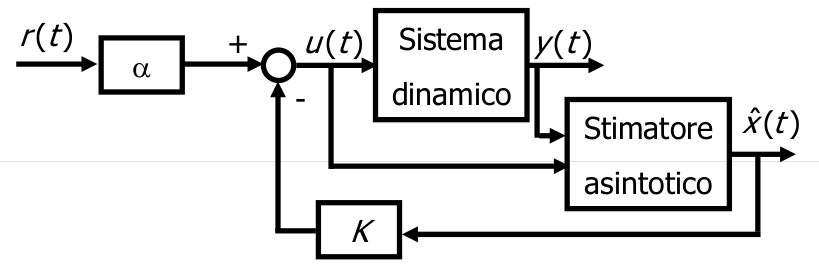
\includegraphics[width=0.5\textwidth]{regolatore-dinamico.png}
    \caption{Regolatore Dinamico}
    \label{fig:regolatore-dinamico}
\end{figure}
L'impianto \`e descritto dalle equazioni:
\[ \begin{system} 
\dot{\vv{x}} = \vv{Ax} + \vv{Bu} \\
\vv{y} = \vv{Cx} + \vv{Du}
\end{system}  \]
Mentre lo stimatore \`e descritto da:
\[ \begin{system} 
    \dot{\hat{\vv{x}}} = \vv{A}\hat{\vv{x}} + \vv{Bu} - \vv{L}(\hat{\vv{y}}-\vv{y}) \\
    \hat{\vv{y}} = \vv{C}\hat{\vv{x}}(\vv{A}-\vv{LC})
\end{system}  \]
% TODO:  <26-04-22, aggiustare tutte le x con il cappello> %
Mettendo tutto insieme, con la legge di controllo $u(t) = -K\hat{x} + \alpha r$, il nuovo sistema \`e composto da $2n$ variabili di stato, dove $n$ sono la variabili dell'impianto, ed $n$ provengono dalle $\hat{\vv{x}}$. Il nuovo sistema regolato \`e descritto come:
\[ \vv{x} _{tot} = \begin{bmatrix} \vv{x} \\ \dot{\vv{x}} \end{bmatrix}  \]
\[ \begin{system} 
\dot{\vv{x}} _{tot} = \vv{A} _{reg}\vv{x} _{tot} + \vv{B} _{reg} \vv{r} \\
\vv{y} = \vv{C} _{reg} \vv{x}_{tot} + \vv{D} _{reg} \vv{r}
\end{system}  \]
Dove:
\begin{table}[H]
    \centering
    \begin{tabular}{cc}
$ \vv{A} _{reg} = \begin{bmatrix}  A & -BK \\ LC & A-BK-LC \end{bmatrix} $ & $ \vv{B} _{reg} = \begin{bmatrix} B \\ B \end{bmatrix} \alpha $ \\ \\
 $\vv{C} _{reg}= \begin{bmatrix} C & -DK \end{bmatrix}$  &  $ \vv{D} _{reg} = \begin{bmatrix} D \end{bmatrix} \alpha $
    \end{tabular}
\end{table}

Scegliendo diverse combinazioni delle variabili di stato \`e possibile ottenere una descrizione da cui sia pi\`u facile ricavare delle informazioni, una scelta \`e ad esempio:
\[ \vv{x} _{tot}  = \begin{bmatrix} \vv{x} \\ \vv{e} \end{bmatrix} \]
\[ \begin{system} 
\dot{\vv{x}} _{tot} = \vv{A} _{reg}\vv{x} _{tot} + \vv{B} _{reg} \vv{r} \\
\vv{y} = \vv{C} _{reg} \vv{x}_{tot} + \vv{D} _{reg} \vv{r}
\end{system} \]
Dove:
\begin{table}[H]
    \centering
    \begin{tabular}{cc}
        $ \vv{A} _{reg} = \begin{bmatrix} A - BK & -BK \\ 0 _{n \times n} & A-LC \end{bmatrix} $ & $ \vv{B} _{reg} = \begin{bmatrix} B \\ 0 _{n \times 1} \end{bmatrix} \alpha $ \\ \\
 $\vv{C} _{reg}= \begin{bmatrix} C-DK & -DK \end{bmatrix}$  &  $ \vv{D} _{reg} = \begin{bmatrix} D \end{bmatrix} \alpha $
    \end{tabular}
\end{table}
Si pu\`o notare che la matrice $\vv{A} _{reg}$ risulta triangolare a blocchi, per cui i suoi $2n$ autovalori sono dati da:
\[ \lambda(\vv{A} _{reg}) = \left\{ \lambda(A-BK) \cup \lambda(A-LC)  \right\}  \]
Questo \`e possibile grazie al teorema di separazione (\ref{the:teorema-di-separazione}).

\begin{theorem}{Teorema Di Separazione}{teorema-di-separazione}
...
\end{theorem}

\subsection{Propriet\`a del Regolatore Dinamico}
La propriet\`a della separazione permette di progettare il sistema in retroazione con la scelta delle matrice $\vv{K}$ e $\vv{L}$ indipendentemente una dall'altra.

Si pu\`o dimostrare che la matrice di trasferimento $\vv{H} _{ry}(s)$ coincide con:
\[ H _{ry}(s) = \left\{ (C-DK) \big[ sI - (A-BK) \big]^{-1} B + D \right\}\alpha  \]
Questo dimostra che le dinamiche associate alla stima dello stato non influenzano il comportamento dell'ingresso.
I poli della funzione di trasferimento sono gli autovalori del sistema, sia della parte \textbf{controllabile} e sia della parte \textbf{osservabile}.



\newpage
\section{Sistemi di Controllo}
In questa sezione il sistema di controllo di riferimento \`e quello nella~\autoref{fig:feedback-control-system}.
\begin{figure}[H]
    \centering
    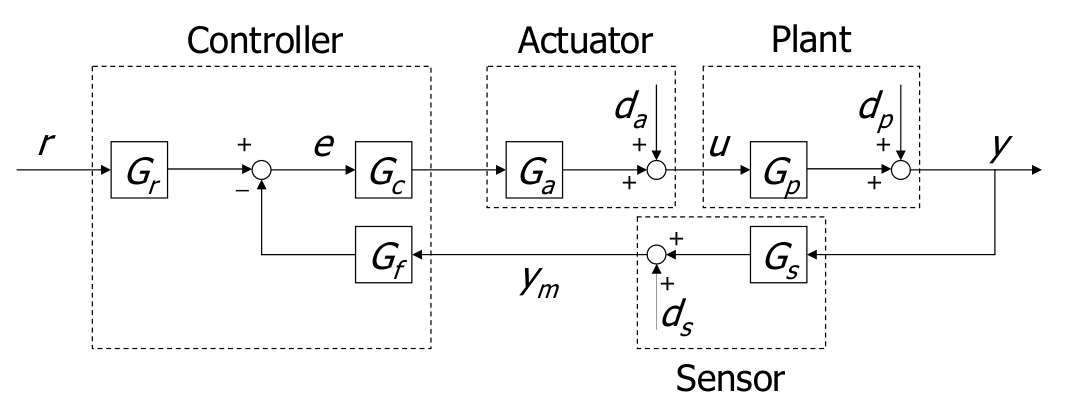
\includegraphics[width=0.8\textwidth]{feedback-control-system.png}
    \caption{Feedback Control System}
    \label{fig:feedback-control-system}
\end{figure}
Gli attuatori mandano i segnali all'impianto, che vengono controllati dai controllori. Un controllore \`e formato da tre parti:
\begin{itemize}
    \item \textbf{prefiltro} ($G_r$): elabora il segnale di riferimento (sar\`a sempre 1);
    \item \textbf{controllore a cascata} ($G_c$);
    \item \textbf{controllore in retroazione} ($G_f$);
\end{itemize}
L'\textbf{anello di controllo} \`e costituito da:
\begin{itemize}
    \item \textbf{catena diretta}: da $G_c$ a $G_p$;
    \item \textbf{catena di retroazione}: $G_s$ e $G_f$;
\end{itemize}
L'obbiettivo principale di progettare un sistema di controllo \`e garantire che il sistema ottenuto sia stabile. In generale all'uscita di ogni blocco vi \`e sommato un rumore.
\begin{definition}{Stabilit\`a Interna di un Sistema di Controllo}{stabilita-interna-di-un-sistema-di-controllo}
    Il sistema di controllo in figura si dice \textbf{internamente stabile} se e solo se l'evoluzione temporale di tutti i segnali sull'anello rimane limitata quando i segnali esterni applicati $(r,\vv{d}_i)$ sono limitati.
\end{definition}
Da questa definizione ne consegue la \textbf{stabilit\`a interna di un sitema di controllo LTI}: \\
Il sistema di controllo LTI sar\`a internamente stabile se e solo se tutte le funzioni trasferimento da tutti i segnali interni all'anello devono essere funzioni di trasferimento BIBO stabili: devono avere poli con parte reale $\Re < 0$.

Calcoliamo la \emph{f.d.t.} tra il segnale di riferimento e l'uscita.
\[ Y(s) = G_p(s)G_a(s)G_c(s) \Big(R(s)G_r(s) - G_f(s)G_sY(s)\Big) \]
\[ Y(s) \Big(1 + G_p(s)G_a(s)G_c(s)G_f(s)G_s(s) \Big) = G_p(s)G_a(s)G_r(s)R(s) \]
\[ \frac{Y(s)}{R(s)} = H _{ry}(s) = \frac{G_pG_aG_cG_r}{1 + \underbrace{G_pG_aG_cG_fG_s}_{L(s)} } = \frac{G_r}{G_fG_s} \frac{L(s)}{1 + L(s)}   \]
La $L(s)$ viene detta \textbf{funzione ad anello} (\ref{def:funzione-ad-anello}).

Adesso si considera il caso in cui tutti gli ingressi del sistema siano spenti tranne $d_p$, allora:
\[ y = d_p + G_pG_aG_c \cdot ( 0 - G_fG_s y) \]
\[ y \cdot (1 + G_pG_aG_cG_fG_s ) = d_p \]
\[ \boxed{ \frac{y}{d_p} = H _{d_p y}(s) = \frac{1}{1+L} }  \]
\`E possibile pensare che tutte le \emph{f.d.t.} del sistema abbiano un termine $1+L$ al denominatore.


\begin{definition}{Funzione ad Anello}{funzione-ad-anello}
    La funzione ad anello viene definito come il prodotto delle \emph{f.d.t.} di tutti i blocchi sull'anello.
    \[ L(s) \triangleq G_1\dots G_n \]
\end{definition}

\begin{definition}{Funzione di Sensitivit\`a}{funzione-di-sensitivita}
    \[ S(s) \triangleq \frac{1}{1+L(s)}  \]
\end{definition}

\begin{definition}{Funzione di Sensitivit\`a Complementare}{funzione-di-sensitivita-complementare}
    \[ T(s) \triangleq 1 - S(s) = \frac{L(s)}{1 + L(s)}  \]
\end{definition}

\`E possibile riformulare il problema, visto che quasi tutte la \emph{f.d.t.} avranno lo stesso denominatore (a meno di cancellazioni), come:
\begin{figure}[H]
    \centering
    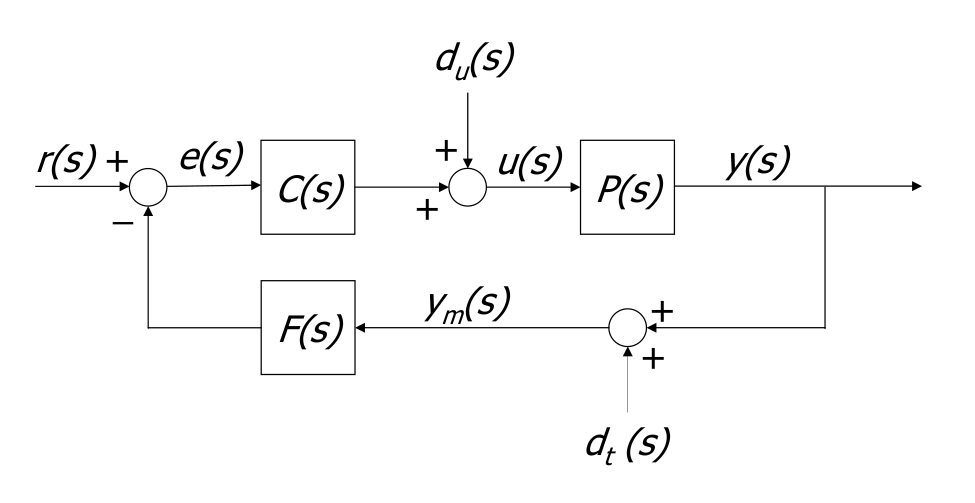
\includegraphics[width=0.7\textwidth]{reduced-control-system.png}
    \caption{Reduced Control System}
    \label{fig:reduced-control-system}
\end{figure}
Le \emph{f.d.t.} del sistema sono discritte da:
\[ \begin{bmatrix} e \\ u \\ y_m  \end{bmatrix} = \frac{1}{1+PCF} \begin{bmatrix} 1 & -PF & -F \\ C & 1 & -CF \\ PC & C & 1 \end{bmatrix} \cdot \begin{bmatrix} r \\ d_u \\ d_t \end{bmatrix}  \]
\begin{theorem}{Interna Stabilit\`a dei Sistemi in Feedback}{interna-stabilita-dei-sistemi-in-feedback}
    Il sistema di controllo \`e internamente stabile se:
    \begin{enumerate}
        \item tutti le radici dell'equazione: $1+L(s) = 0$ devono avere parte reale $< 0$;
        \item non ci devono essere cancellazioni in $\Re[s] \geqslant 0$ quando si forma il prodotto $PCF$: quando avvengono i prodotti dei numeratori e dei denominatori, se alcuni denominatori delle \emph{f.d.t.} hanno dei poli a parte reale $\Re > 0$ e questi vengono cancellati con uno zero in uno dei numeratori, il teorema non \`e pi\`u valido.
            \[ L = G_1 G_2 \dots G_n \]
            \[ L = \frac{N_1}{D_1} \frac{N_2}{D_2} \dots \frac{N_n}{D_n} \]
    \end{enumerate}
\end{theorem}

Cosideriamo un impianto instabile $G_p = \frac{N_p(s)}{D_p(s)} $, in alcuni casi \`e necessario realizzare un controllore che anche esso sia instabile, descritto da $G_c = \frac{N_c(s)}{D_c(s)}$. Anche se $L(s)$ possiede dei dei poli a parte reale positiva, il motivo per il sistema di controllo risulta stabile \textbf{senza elidere i poli}, \`e dato dal fatto che si deve fare riferimento alla funzione $1 + L(s) = 0$, che risulter\`a:
\[ 1 +  G_c(s)G_p(s) = 1 + \frac{N_c(s)}{D_c(s)} \frac{N_p(s)}{D_p(s)} = 0  \]
Che pu\`o essere riscritta come:
\[ \frac{ \overbrace{D_cD_p + N_cN_p}^{\text{poli della \emph{f.d.t.} }} }{D_cD_p}  \]
\[ \frac{L}{1 + L}  = \frac{\frac{N_L}{D_L} }{\frac{D_L + N_L}{D_L} } = \frac{N_L}{D_L+N_L} \]
Dove i poli del sistema di controllo sono dati da $D_cD_p + N_cN_p$, e non dai poli di $L(s)$, ecco il motivo per cui non \`e necessario elidere i poli a parte reale positiva per rendere il sistema stabile, oltre a violare la seconda condizione del Teorema (\ref{the:interna-stabilita-dei-sistemi-in-feedback}).



\subsection{Contour Mapping}
Il signor Nyquist us\`o il teorema di Cauchy, per stabile un criterio per determinare la stabilit\`a di un sistema di controllo.

Si definisce nel piano della variabile $s = \sigma + j\omega$ una funzione che mappa due valori $u$ e $v$ sul piano complesso: $F(s) = u + jv$, la seguente mappatura viene applicata ad un curva chiusa $\Gamma_s : \RR \to \mathbb{C}$, tale che l'immagine \`e della nuova curva \`e data da $\Gamma_F = F \circ \Gamma_s$.

\begin{theorem}{Cauchy's Argument Principle}{cauchys-argument-principle}
    Se consideriamo una curva $\Gamma_s$ chiusa percorsa in senso orario nel piano di $s$ allora, nel piano di $F(s)$ si ottiene un'altra curva chiusa $\Gamma_F = F(\Gamma_s) = \left\{ F(s) : s \in \Gamma_s \right\}$, percorsa in senso orario, che andr\`a a encircolare l'origine un numero $N$ di volte dove $N = Z - P$, con:
    \begin{itemize}
        \item $Z$: numero di zeri di $F(s)$ encircolati da $\Gamma_s$ in $s$;
        \item $P$: numero di poli di $F(s)$ encircolati da $\Gamma_s$ in $s$;
        \item non attraversa l'origine;
    \end{itemize}
\end{theorem}

\begin{example}{}{}
    Prendiamo $F(s)$ con due poli e due zeri. Allora:
\[ F(s) = |F(s)| \angle(s+z_1) + \angle(s+z_2) - \angle(s+p_1) - \angle(s+p_2)  \]
\[ F(s) = |F(s)| \angle(\phi _{z_1} + \phi _{z_2} - \phi _{p_1} - \phi _{p_2})\]
\[ F(s) = |F(s)| \angle\phi_F \]
\begin{figure}[H]
    \centering
    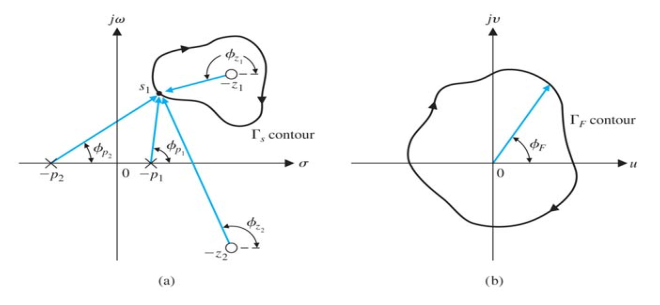
\includegraphics[width=0.8\textwidth]{encircolamento-esempio.png}
    \caption{Encircolamento Esempio}
    \label{fig:encircolamento-esempio}
\end{figure}
Il contributo totale dato da $p_1$, $p_2$ e $z_2$ all'anglolo $\phi_F$ \`e nullo. Dunque $\phi_F$ deve necessariamente compiere un giro di $360^{\circ}$ dato dal contributo di $z_1$.
\end{example}

Questo teorema \`e importante per stabilire la stabilit\`a dei sistemi in retroazione.

Possiamo applicare il teorema di Cauchy nel modo seguente: si prende la curva di Nyquist $\Gamma_s = \Gamma_N$ che viene mappata su: $F(s) = 1 + L(s)$. Dal momento che $L(s) = F(s) - 1$ dove il numero di circolamenti passa daessere centrati nell'origine nel punto $-1 + j0$; il numero di $Z$ deve essere 0 per garantire la stabilit\`a, il motivo \`e che la curva di Nyquist $\Gamma_N$ contorna tutto il piano $\Re \geqslant 0$, dunque se $Z$ \`e diverso da 0, vuol dire che $1 + L(s)$ presenta una radice a parte reale positiva, che andrebbe a violare il teorema (\ref{the:interna-stabilita-dei-sistemi-in-feedback}).

\begin{theorem}{Nyquist's Criterion}{nyquists-criterion}
    Data un \textbf{Contorno di Nyquist} $\Gamma_s$, sia $P$ il numero di poli di $L(s)$ encircolati da $\Gamma_s$, e $Z$ il numero di zeri di $1 + L(s)$ encircolati da $\Gamma_s$. Se $Z$ \`e il numero di poli di un sistema chiuso in feedback sulla parte destra del piano, e $P$ \`e il numero di poli di una \emph{f.d.t.} ad anello aperto $L(s)$ nella parte destra del piano, il contorno risultante nel $L(s)$-piano, $\Gamma _{L(s)}$ deve encircolare in senso orarioil punto $(-1 + j0)$ $N$ volte, tale che $N = Z - P$.

    Si assuma che il diagramma di Nyquist di $L(j\omega)$ non attraversi il punto $-1+j0$. Il numero $P _{cl}$ (closed loop) di radice a parte reale positiva dell'equazione $1 + L(s) = 0$ \`e dato da:
    \[ P _{cl} = P _{ol} +  N \]
    Dove:
    \begin{itemize}
        \item $P _{ol}$: (open loop) \`e il numero di poli a parte reale strettamente positiva di $L(s)$;
        \item $N$: \`e il numero di encircolamenti del diagramma di Nyquist di $L(j\omega)$ attorno al punto $-1 +j0$, calcolati come la differenza tra il numero di giri in senso orario ed antiorario;
    \end{itemize}

    Se il diagramma di Nyquist attraversa il punto $-1 +0j$, allora: l'equazione $1 + L(s) = 0$ ha una radice immaginaria.

    In colcusione:
    \[ \#\text{Poli instabili di }L(s) = \]
\[ = \#\text{Poli instabili di }\frac{1}{1 + L(s)} + \#\text{Encircolamenti antiorari di -1 da } L\circ\Gamma_N \]
\end{theorem}

\begin{theorem}{Stabilit\`a BIDO dei Sistemi in Feedback}{stabilita-bido-dei-sistemi-in-feedback}
    Si assuma che $F^{-1}(s)$ sia BIBO stabile. Allora le seguenti condizioni sono equivalenti:
    \begin{itemize}
        \item $N = -P _{ol}$;
        \item tutte le radici dell'equazione $1 + L(s) = 0$ hanno parte reale negativa;\
        \item il sistema in feedback \`e BIBO stabile;
    \end{itemize}
\end{theorem}

Se il sistema ad anello aperto \`e instabile in origine, \`e necessario creare un sistema in feedback per stabilizzarlo.

\begin{example}{}{}
    \[ L(s) = \frac{1}{s^{2} + 3s + 2}  \]
    La funzione ad anello apero non ha poli a parte reale negatva, $P _{ol} = 0$:
    \[ L(s) = \frac{1}{2} \frac{1}{\left( 1 + \frac{s}{2}  \right) \left( 1 + s \right)  }  \]
    Entrambi i poli sono stabili. Se ora prendiamo il diagramma di Nyquist di $L$ vediamo che il punto -1 non viene mai encircolato, $N = 0$:
    \begin{figure}[H]
        \centering
        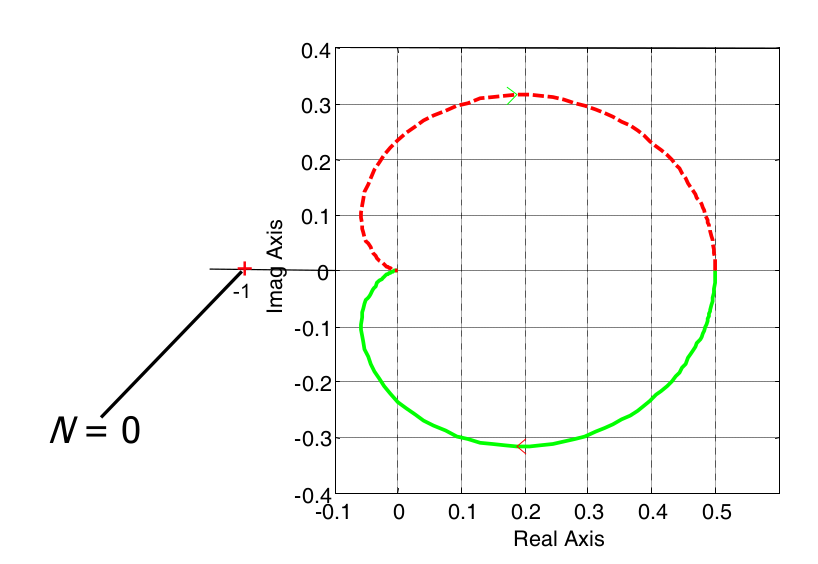
\includegraphics[width=0.4\textwidth]{diagramma-di-nyquist-esempio.png}
        \caption{Diagramma Di Nyquist Esempio}
        \label{fig:diagramma-di-nyquist-esempio}
    \end{figure}
    In conclusione il numero di poli instabili della funzione closed loop sono:
    \[ P _{cl} = P _{ol} + N = 0 + 0 = 0 \]
    Il sistema \`e stabile.
\end{example}

\subsection{Struttura di un Controllore}
Per avere un sistema stabile si deve avere che, per tutti i disturbi e gli ingressi limitati, la risposta del sistema in ogni punto dell'anello di controllo deve essere finita. \`E possibile avere un sistema internamente instabile ma che abbia una \emph{f.d.t.} stabile, quindi che sia \textbf{input-output stable}. Questo avviene quando il sistema ha dei modelli instabili nascosti. Inoltre un boun sitema retroazionato deve forinre un buon \textbf{tracking trasitorio} ed un opportuno \textbf{stato stazionario}, generalmente non \`e possible un buon tracciamento per un qualsiasi segnale, questo \`e il motivo per cui si usano solo dei segnali o delle classi di segnali speicifi.

\subsection{Stabilit\`a Relativa}
...

\subsection{Risposta Stazionaria}
Ora studiamo il il comportamento del sistema di controllo quando vogliamo imporre il comportamento del segnale di riferimento alla risposta a steady-state del sitema. Per fare ci\`o apportiamo delle modifiche al sistema di controllo pi\`u generale in figura~\autoref{fig:feedback-control-system}, senza perdere di generalit\`a, assumiamo che:
\begin{itemize}
    \item $G_r = 1$;
    \item $G_a =$ const: larga banda a causa da una dinamica veloce;
    \item $G_f =$ const: controllare il guadagno della risposta stazionaria;
    \item $G_s = $ const: larga banda a causa da una dinamica veloce;
\end{itemize}

Nella struttura della \emph{f.d.t.} di un controllore, il denominatore deve avere grado maggiore o uguale a quello del numeratore, in caso contrario il sistema prevede il futuro. La \emph{f.d.t.} del controllare \`e possibile rappresentarla nella seguente forma:
\begin{definition}{Controllore}{controllore}
\[ G_c (s) = \frac{K_c}{s^{\nu}} \prod_{i}^{}   \underbrace{\left( \frac{1 + \frac{s}{z _{di}} }{1 + \frac{s}{m _{di} z _{di}} }   \right)}_{LEAD} \prod_{j}^{}   \underbrace{\left( \frac{ 1 + \frac{s}{m _{ij} p _{ij}} }{ 1 + \frac{s}{p _{ij}} }  \right)}_{LAG} \]
\end{definition}

Il primo blocco della \emph{f.d.t.} \`e detta rete \textbf{derivativa} (o \textbf{anticipatrice} o \textbf{LEAD}), dove il coefficente $m _{di}$ \`e sempre $> 1$, la rete LEAD \`e una rete con la frequenza dei poli sempre maggiore di quella degli zeri.

Il secondo blocco rappresenta una rete \textbf{integrativa} (o \textbf{attenuatrice} o \textbf{LAG}), nella quale lo zero \`e a frequenza pi\`u alta del polo, perch\`e $m _{ij}$ \`e sempre $> 1$.

Si definiscono i guadagni:
\begin{definition}{Guadagno Controllore}{guadagno-controllore}
\[ K_c = \lim_{s \to 0^{+}}  s^{\nu} G_c(s) \]
\end{definition}
\begin{definition}{Guadagno Impianto}{guadagno-impianto}
\[ K_p = \lim_{s \to 0^{+}} s^{p}G_p(s)\]
\end{definition}

Il progetto di un controllore deve soddisfare delle specifiche, le pi\`u importanti sono:
\begin{itemize}
    \item La stabilizzazione di un sitema instabile;
    \item L'inseguimento di un segnale di riferimento;
    \item ...
\end{itemize}

\subsection{Segnali Polinomiali}
I segnali polinomiali sono una classe di segnali che vorremmo fossero inseguiti, della forma:
\[ r(t) = R_0 \frac{t^{h}}{h!}\varepsilon(t) \quad\longrightarrow\quad r(s) = R_0 \frac{1}{s^{h+1}}  \]
Si vogliono calcolare le \textbf{prestazioni relative} al tracking del segnali di riferimento, si definisce l'errore di uscita:
\begin{definition}{Errore Relativo di Tracking}{errore-relativo-di-tracking}
    \[ e_r(t) = y_r(t) - y_d(t) = y_r (t) - K_dr(t) \]
\end{definition}



L'obbiettivo fondamentale del progetto \`e garantire l'inseguimento del riferimento, anche in presenza di segnali in ingresso esterni, per questo se definsce lo \textbf{steady-state tracking error}, che ci da una misura di quanto bene l'uscita sta inseguende il riferimento in risposta permanente.
\begin{definition}{Steady-State Tracking Error}{steady-state-tracking-error}
    \[ e _{r}^{\infty} = \lim_{t \to \infty} e_r(t) \]
\end{definition}

Si considera per primo il segnale di riferimento, successivamente si considerano i segnali di disturbo uno ad uno modificando di conseguenza il controllore, usando la sovrapposizione degli effetti.
\[ e_r^{\infty} = \lim_{s \to 0} se_r(s) = \lim_{s \to 0} s(y_r(s) - K_dr(s))  \]
\begin{theorem}{Specifiche per Fattore di Scala}{specifiche-per-fattore-di-scala}
    \[ K_d = \frac{1}{G_fG_s}  \]
\end{theorem}

Vediamo come \`e fatto $y_r$ (solo con $r$ acceso):
\[ y_r(s) = G _{ry}(s) \cdot r(r) \]
\[ e_r(s) = \frac{G}{1 + GH} r(s) - K_dr(s) \]
\[ \frac{G}{1 + GH}  = \frac{\frac{L}{H} }{1 + L} =  \frac{1}{H} T = \frac{1}{G_sG_f} T \]

\[ y_r(s) = T \frac{1}{G_sG_f} r(s) \]
Cosa accade quando mandiamo in ingresso un segnale a gradino $r(t) = R_0 \to r(s) = \frac{R_0}{s}$, usiamo il teorema del valore finale per risolvere l'equazione (\ref{the:teorema-del-valore-finale}):
\begin{align*}
y_r^{\infty} & = \lim_{t \to \infty} y_r(t) = \lim_{s \to 0} sy_r(s) \\
& = \lim_{s \to 0} s T(s) \frac{1}{G_sG_f} \frac{R_0}{s} = \\
& = T(0) \frac{1}{G_sG_f} R_0 
\end{align*}
Supponiamo che $\nu + p > 0$, allora $T(s) \underset{s \to 0}{\longrightarrow} 1$. L'uscita in regime permanete vale:
\[ \boxed{y_r^{\infty} = R_0 \frac{1}{G_sG_f} = R_0 K_d} \]
Consideriamo ora l'uscita in presenza di un qualunque riferimento polinomiale.
\[ H = G_sG_f = \frac{1}{K_d} \]
\[ e_r(s) = \frac{G}{1 + GH}  r(s) - K_dr(s) \]
\[ \boxed{ e_r(s) = \frac{K_d^{2}}{K_d + G} r(s) } \]
Posso scrivere la trasformata del mio errore come:
\begin{align*}
e_r^{\infty} & = \lim_{s \to 0} s (y_r(s) - K_dr(s)) = \\
     & = \lim_{s \to 0} s \frac{K_d^{2}}{K_d + G} r(s) = \\
     & = \boxed{\lim_{s \to 0} s\frac{K_d^{2}}{K_d + G_c(s)G_p(s)G_a} \cdot \frac{R_0}{s^{h+1}} }
\end{align*}
Analizziamo chi sono $G_p$ e $G_c$.

Quando $s$ tende a zero la parte LEAD e la parte LAG tendono a 1, dunque:
$G_p = \frac{K_c}{s^{\nu}} $.
Ma anche $G_p$ ha una forma simile, dunque per $s$ che tende a 0: $G_p = \frac{K_p}{s^{p}} $.

Dunque:
\[ e_r^{\infty} = \lim_{s \to 0} s \frac{K_d^{2}}{K_d + \frac{K_c}{s^{\nu}} \frac{K_p}{s^{p}} G_a } \frac{R_0}{s^{h+1}}   \]\

\[ e_r^{\infty} = \lim_{s \to 0}  \frac{s^{\nu+p}K_d^{2}}{s^{\nu+p}K_d + K_cK_pG_a} \frac{R_0}{s^{h}} \]
\begin{theorem}{Specifiche per Riferimento Polinomiale}{specifiche-per-riferimento-polinomiale}
    \[ e_r^{\infty} = \begin{system} 
    0 & \nu+p > h \\
    \frac{K_d^{2}R_0}{\beta K_d + K_cK_pG_a} & \nu+p = h
    \end{system}  \]
    \[ \beta  = 1\;(\text{se }\nu + p = 0) ;\quad \beta = 0\; (\text{se }\nu + p > 0)  \]
    \end{theorem}
Si possono prendere due strade:
\begin{itemize}
    \item $|e_r^{\infty}| = 0$: L'errore relativo tende a 0: si deve imporre $\nu + p > h$ (che sono decisi da noi);
    \item $|e_r^{\infty}| < \rho$: L'errore relativo \`e minore di una certa costante.
\end{itemize}

Consideriamo ora gli effetti dati dai segnali di disturbo. Consideriamo la classe dei disturbi polinomiali:
\[ \boxed{ d(t) = D_0 \frac{t^{h}}{h!} \overset{\LL}{\longrightarrow} D_0 \frac{D_0}{s^{h+1}} }  \]
I disturbi entrano direttamente nella catena, non sono decisi da noi e per questo non sono controllabili. Usando il metodo della sovrapposizione degli effetti possiamo chiudere tutti gli altri segnali di ingresso (compresi i disturbi) e studiarli singolarmente uno per  uno. Il nostro compito sar\`a quello di limitare l'effetto che il disturbo comporta sull'uscita, idealmete portandolo a 0. Come vedremo lo studio dei segnali di disturbo non ha delle regole ben precise, sar\`a dunque necessario calcolare la \emph{f.d.t.} per ogni disturbo.

Facalizziamoci sull'errore di uscita $d_p$ (spegnendo gli altri segnali), \\ idealmente (avendo anche il riferminto a 0), l'uscita deve rimanere a 0:
\[ e_{d_p}(t) = y_{d_p}(t) \]
L'errore a steady-state \`e dato da:
\[ e_{d_a}^{\infty} = \lim_{t \to \infty} e_{d_p}(t) \]
Anche in questo caso usiamo il teorema del valore finale:
\begin{align*}
    e_{d_p}^{\infty} &= \lim_{t \to \infty} e_{d_p}(t) = \\
    & = \lim_{s \to 0} sy _{d_p}(s) = \\
    & = \lim_{s \to 0} s\frac{1}{1+L(s)} d_p(s) = \\
    & = \lim_{s \to 0} s\frac{s^{\nu+p}}{s ^{\nu+p} + K_cK_pG_aG_fG_s} \frac{D_{p0}}{s^{h+1}} = \\
    \\
    & = \begin{system} 
        0 & \nu+p > h \\
        \frac{D_{p0}}{\beta + K_cK_pG_aG_fG_s} & \nu+p = h
    \end{system} 
\end{align*}

\newpage
\begin{problem}{Problema 1}{problema-1}
    Costruire un controllore rispettando le specifiche.
    \[ G_p(s) = \frac{25}{s^{3} + 3.3s^{2} + 2s}  \]
    Il sitema ha i seguenti valori per i disturbi e le \emph{f.d.t.} :
    \begin{figure}[H]
        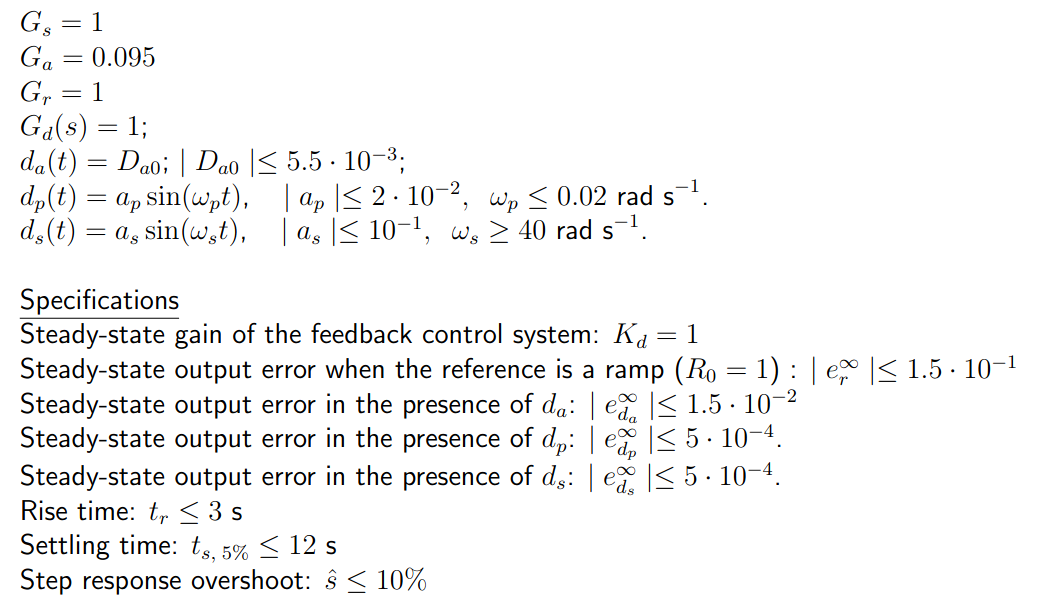
\includegraphics[width=0.9\textwidth]{dati-problema-1.png}
    \end{figure}

    1. Partiamo dalla specifa che $K_d = 1$, sappiamo che $K_d = \frac{1}{G_fG_s}$, a patto che $\nu + p > 0$, se non fosse cos\`i il tipo del sistema \`e uguale a 0, allora in uscita ottengo un errore. Prima di poter applicare quella formula si deve andare a verificare se quella condizione \`e verificata. $p$ \`e ugaule a 1, allora sicuramente $p + \nu$ \`e maggiore di 0:
    \[ K_d = \frac{1}{G_fG_s} \implies G_f = \frac{1}{G_sK_d}  = 1 \]

    2. Troviamo per come primo punto il valore di $\nu$; si ha dalla formula (\ref{the:specifiche-per-riferimento-polinomiale}) che: $p$ ha valore 1, infatti:
    \[ G_p = \frac{1}{s} \frac{25}{s^{2} + 3.3s + 2}  \]
    Per ottenere un errore reltivo in modulo minore di una certa costante, deve essere vero che: $\nu + p = h$, dove $h$ \`e l'ordine del polinomio di riferimento, che in questo caso \`e $1$, visto che $r$ \`e una rampa. Dunque abbiamo che: $\nu = h - p = 0$. Allora se $\nu + p \neq 0$, $\beta$ \`e uguale a 0, dunque si trova il vincolo su $K_c$:
    \[ K_p = \lim_{s \to 0} sG_p(s) = 12.5 \]

    \begin{align*}
        \left| e_r^{\infty} \right| & = \left|\lim_{t \to \infty}  y(t) - K_dr(t) \right| = \\
        & = |\lim_{s \to 0} s\cdot[y(s) - K_dr(s)]| = \\
        & = |\lim_{s \to 0} s\cdot[G _{ry}(s)r(s) - K_dr(s)]| = \\
        & = \left|\lim_{s \to 0} s\cdot \left[\frac{L}{1+L} \frac{1}{G_fG_s} r(s) - K_dr(s)\right] \right| = \\
        & = \left|\lim_{s \to 0} s\cdot\frac{K_d^{2}s^{\nu + 1}}{s^{\nu + 1}K_d + K_pK_cG_a } \frac{R_0}{s^{2}} \right| = \\
        & = \left| \frac{K_d^{2}R_0}{K_cK_dG_a}  \right|  \\
        \\
        \implies & \left| \frac{K_d^{2} R_0}{ K_c K_p G_a} \right|  < 0.15 \\
        & \left| K_c \right| > \frac{1}{0.15} \left| \frac{K_d^{2} R_0}{ K_p G_a} \right|  \\
        & \left| K_c \right|  > 5.61 
    \end{align*}

    3. Otteniamo le specifiche per il segnale $e _{d_a}(t)$:
    \begin{align*}
        \left| e _{d_a}^{\infty} \right| & = \lim_{t \to \infty} |e _{d_a}(t)| =| \lim_{s \to 0}  s e _{d_a}(s)| = \\
        & = \lim_{s \to 0}  |s y _{d_a}(s)| = \\
        & = \lim_{s \to 0} | s G _{d_ay} d_a(s) | = \\
        & = \lim_{s \to 0} \left| s \frac{G_p}{1 + L} d_a  \right|  = \\
        & = \lim_{s \to 0} \left|  s \frac{\frac{K_p}{s} }{1  +\frac{K_p}{s} \frac{K_c}{s^{\nu}} G_aG_fG_s } \frac{D_{a0}}{s}  \right| \\
        & = \lim_{s \to 0} \left|  \frac{s^{\nu}K_dK_pD_{a0}}{s^{\nu+1}K_d + K_pK_cG_a} \right| = \\
        & = \left| \frac{K_dD _{a0}}{K_cG_a}  \right| 
    \end{align*} 
    Anche in questo caso ottenimo una specifica per $\nu$ pari a 0, per ottenere un errore in feriore ad un costante.
    \[ \left|  \frac{K_d D _{a0}}{K_cG_a} \right| < 1.5 \cdot 10^{-2} \]
    \[ \left| K_c \right|  > 3.86 \]
    Sommario:
    \begin{enumerate}
        \item $G_f = 1$;
        \item $\nu = 0;\quad |K_c| > 5.61$;
        \item $\nu = 0;\quad |K_c| > 3.86$;
    \end{enumerate}
    Ricavo che:
    \[ \boxed{\nu = 0;\quad |K_c| > 5.61} \]
    
\end{problem}


\newpage
\section{Risposta in Frequenza}
Si pu\`o verificare che, per un sisetma di controllo generico, il contributo dei rumori nella catena diretta risultano:
\[ y(s) = T(s) \frac{1}{H}  r(s) + S(s)d_p(s) + G_p(s)S(s) d_a(s) - T(s) \frac{1}{G_s} d_s(s) \]
Ideamente si vuole che in un sistema, $T(s)$ sia uguale ad 1. Se ci\`o fosse vero allora, $S(s)$ sarebbe ugale a 0, dunque l'uscita risulta proprio uguale a (considerando $H = 1$):
\[ y(s) = r(s) - \frac{1}{G_s} d_s(s)\]
L'unico termine che causa dei problemi \`e dato dal rumore causato dal sensore. Sorgono dei problemi, uno di questi \`e che se $T$ fosse 1, $L$ dovrebbe tendere ad infinito, ma questo non \`e realizzabile in un sistema fisico, inoltre non \`e possibile attenuare i disturbi senza l'incorretto inseguimento del riferimento, oltre al fatto che anche se $T(s)$ fosse sempre 1, si avrebbero comunque dei  termini dati dal rumore che non scompaiono.

Per risolvere questo problema devo confrontare $r(s)$ e $d_s(s)$, guardando il problema nella sua risposta in frequenza riesco a risolvere il problema inseguendo il rifermento ed attenuare i disturbi. Infatti si pu\`o porre $T(j\omega)$ a 1 nella banda di $r(s)$ e a 0 nella banda dei disturbi $d_s$.


Vogliamo che la funzione $|T(j \omega)|$ sia ugale a $0dB$ nel range della benda del riferimento. Per $\omega$ maggiore della banda del riferimento, si vuole che il modulo sia 0. Un buon progetto ha una funzione simile alla forma nella~\autoref{fig:buon-progetto}. Per $S$ si vuole che a bassa frequenza si il suo modulo valga 0, per ridurre i disturbi.
\begin{figure}[H]
    \centering
    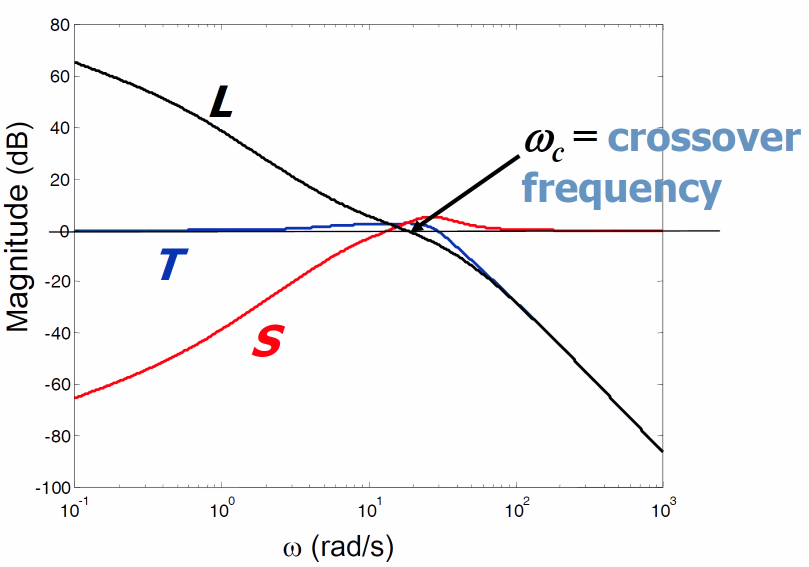
\includegraphics[width=0.5\textwidth]{buon-progetto.png}
    \caption{Buon Progetto}
    \label{fig:buon-progetto}
\end{figure}


Il comportamento nell media frequenza:
\begin{definition}{Media Frequenza}{media-frequenza}
    Anche detta \textbf{crossover frequency}, e la frequenza tale per cui:
    \[ \omega_c: |L(j\omega_c)| = 1 = 0dB \]
\end{definition}

Per la frequenza di crossover il modulo di $T$ ed il modulo di $S$ hanno lo stesso valore. Sul diagramma di Nyquist il punto nella frequenza di $\omega_c$ il valore del vettore \`e proprio 1. Se per qualche motivo la funzione ad anello encircola il punto $-1+j0$ (sistema diventa instabile), allora devo, in qualche modo, modificare la funzione ad anello in un intorno della frequenza di crossover.

Un comportamento ragionevole della funzione ad anello \`e: a 0 vale infinito, e decresce fino a raggiungere 0, vicino l'attraversamemnto della frequenza di crossover la sua fase deve trovarsi ad una distanza ragionevole da $-180^{\circ}$, se cos\`i non fosse ci sarebbe un attraversamemnto del punto a $-1+j0$.

Consideriamo disturbi sinusoidali che entrano direttamente \\ nell'anello di retroazione. Le funzioni sinusoidali non hanno limite per $t$ che tende a infinto, non si pu\`o applicare il limite del valore finale, \`e per questo motivo che si una il teorema della risposta armonica.
\begin{theorem}{Teorema della Risposta Armonica}{teorema-della-risposta-armonica}
    Supponendo che $H(s)$ sia la \emph{f.d.t.} di un sistema lineare, allora dato $Y(s) = H(s)X(s)$:
    \[ x(t) = a_x\sin(\omega_xt + \phi_x) \implies y(t) = a_x |H(j\omega_x)| \sin(\omega_xt + \phi_x + \angle H(j\omega_x)) \]
\end{theorem}

Supponiamo di voler ridurre il rumore causato dal sensore:
\[ |e _{d_s}^{\infty}| = \left| y _{d_s}^{\infty} \right| < \rho_d \]

La specifica di prestazione relativa alle sinusoidi \`e:
\[ \left| e_{d_s}^{\infty} \right| < \rho_s   \]
\[ \implies \left| a_s |T(j\omega_s)|\frac{1}{G_s} \sin(\omega_st + \phi_s) \right| < a_s |T(j\omega_s)|\frac{1}{G_s} < \rho_s \]
Per $L(j\omega) << 1$, la $T(j\omega)$ ha valori molto simili, infatti si ha che $T(j\omega) \simeq L(j\omega)$, allora:
\[ \boxed{|L(j\omega_s)| < \frac{\rho_sG_s}{a_s} = M_T^{HF} \qquad \forall \omega_s > \omega_s^{-}} \]

Viene naturale fissare una soglia minina di frequenze $\omega_s^{-}$, oltre il quale si vuole che la funzione $T$ sia inferiore di un certo valore.

Il primo vincolo \`e quello su $\omega_c$, definta la $\omega_H$ potrei sceglire come vincolo $\omega_c < \omega_H$

Un progetto fatto bene vuole che $L$ passi in $\omega_c$ esattamnte che una una pendenza di $-20dB/dec$. Il motivo per cui non si pu\`o scendere pi\`u velocemente \`e che se la pendenza \`e troppo ripida abbiamo pi\`u poli nell'origine, questo corrispode ad un contributo nella fase di $-90^{\circ}$ per ogni polo, come abiamo visto ad un certo punto ho bisogno di far salire la fase vicino all'intorno a $\omega_c$ con degli zeri, altrimenti il sitema non \`e stabile per il criterio di Nyquist (\ref{the:nyquists-criterion}), dunque \`e conveniente prendere i valori di $\nu$ pi\`u bassi.

Per questa ragione \`e parsimonioso prendere come vincolo:
\[ \omega_c \leqslant \frac{\omega_H}{2}  \]
A meno che non si arriva sullo spigolo con una fase minore, in quel caso si ha pi\`u margine per scegliere il vincolo.

Consideriamo ora l'attenuazione di un disturbo sinusoidale che entra nella catena diretta. Consideriamo il disturbo $d_p = a_p\sin(\omega_pt),\quad \forall \omega_p < \omega_p^{+}$.

Come prima utilizziamo il teomrema della risposta armonica:
\[ |e_{d_p}^{\infty}| = |y _{d_p}^{\infty}| =  \big| a_p|S(j\omega_p)|\sin(\omega_pt + \phi_p) \big| < \rho_p  \]
Allora:
\[ \implies |S(j\omega_p)| < \frac{\rho_p}{a_p} = M_S^{LF} \qquad \forall \omega_p < \omega_p^{+} \]

\[ \implies |L(j\omega_p)| > \frac{a_p}{\rho_p} \qquad \forall \omega_p < \omega_p^{+} \]

Anche in questo caso possiamo trovare un costante $\omega_L$, tale che:
\[ \omega_c \geqslant  2\cdot\omega_L \]

In coclusione ho dei vincoli dati da $T$ e da $S$, che impongono di scegliere una $\omega_c$ all'interno di un intervallo, che sar\`a che avr\`a come esteremi i limiti sulle alte frequenza e sulle basse frequenze, tale frequenza sar\`a detta \textbf{frequenza di crossover desiderata}.
\[ \omega_{c,des} \in \left[ 2\omega_L, \frac{\omega_H}{2}  \right] \]

Se dovesse accadere che $2\omega_L > \frac{\omega_H}{2}$, le specifiche sono conflittuali, ci\`o vuol dire che il problema di controllo non ha soluzione.



\newpage
\section{Specifiche per Transitorio}
Prendiamo in esame le specifiche per il transitorio. Come abbiamo gi\`a visto, il transitorio \`e sempre presente in un sistema e non si pu\`o eliminare. Una situazione tipica \`e la seguente:
\begin{figure}[H]
    \centering
    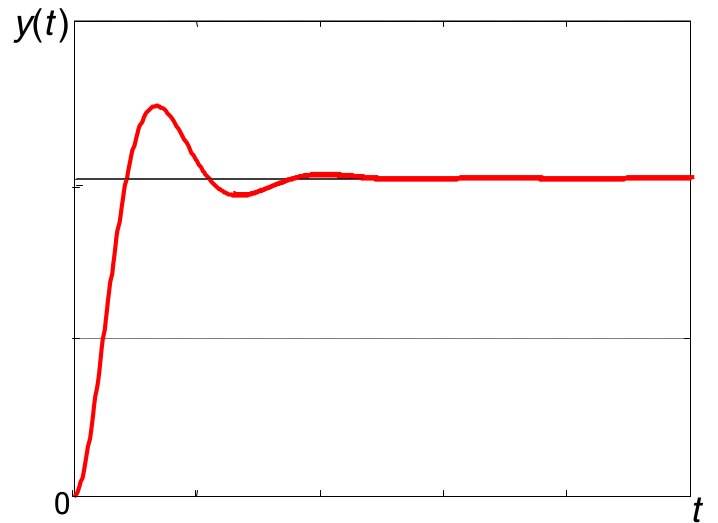
\includegraphics[width=0.4\textwidth]{transitorio-di-un-sistema.png}
    \caption{Transitorio Di Un Sistema}
    \label{fig:transitorio-di-un-sistema}
\end{figure}
Per analizzare il comportamento del transitorio si manda in entrata un segnale gradino unitario e si definiscono delle grandezze a partire dall'uscita:
\begin{definition}{Maximum Overshoot}{maximum-overshoot}
    Anche detta \textbf{massima sovraelongazione}, \`e definita come:
    \[ \hat{s} = \frac{y _{max} - y _{\infty}}{ y _{\infty}}  \]
    Questa quatit\`a puo essere anche definita in percentuale:
    \[ \hat{s}_{\%} = 100\cdot \hat{s} \]
\end{definition}

\begin{definition}{Rise Time}{rise-time}
    Il \textbf{tempo di salita}: $t_r$ \`e definito come il tempo richesto per arrivare dallo $0\%$ al $100\%$ del valore in regime stazionario.
\end{definition}

\begin{definition}{10\%-90\% Rise Time}{10-90-rise-time}
    $t_s'$ \`e definito come il tempo richiesto per arrivare dal $10\%$ al $90\%$ del valore a regime staizionario.
\end{definition}

\begin{definition}{Settling Time}{settling-time}
    Il \textbf{tempo di assestamento} $ \pm \alpha * 100\%$: $t _{s,\alpha\%}$ tale per cui:
    \[  \| y(t) - y _{\infty} \|_{\infty}  < \alpha \cdot y _{\infty} \qquad \forall t > t _{s,\alpha\%} \]
\end{definition}

Si definiscono delle specifiche per ogni tipologia di segnale e durante il progetto si deve garantire il rispetto di tali costanti:
\[ \boxed{ \hat{s} \leqslant \bar{\hat{s}};\qquad t_r \leqslant \bar{t}_r;\qquad t_{s,\alpha\%} \leqslant \bar{t}_{s,\alpha\%} } \]

In generale non si conosce la struttura di $T$. Per studiare il i criteri sopra descritti facciamo un assunzione molto forte su quello che \`e la struttura di $T$. La assumiamo come una funzione a poli complessi coniugati, detta \textbf{funzione prototipo del secondo ordine}:
\[ y(s) = T(s) \cdot \underbrace{\frac{1}{G_fG_s}}_{K_d} \cdot r(s) \]
\[ T(s) = \frac{1}{\displaystyle 1 + \frac{2\zeta}{\omega_n} s + \frac{s^{2}}{\omega_n^{2}} }  \]
I vantaggi di usare qeusta rappresentazoine sono:
\begin{itemize}
    \item guadagno stazionario;
    \item non ha zeri, 2 poli complessi coniugati;
        \[ 0 < \zeta \leqslant 1 \]
\end{itemize}
La risposta al gradino unitario \`e data da:
\[ y(t) = 1 - \frac{e^{-\zeta\omega_n t}}{\sqrt{1-\zeta^{2}}} \sin\left( \omega_n t + \arctan \left( \frac{\sqrt{1-\zeta^{2}}}{\zeta}  \right)  \right)   \]
\begin{figure}[H]
    \centering
    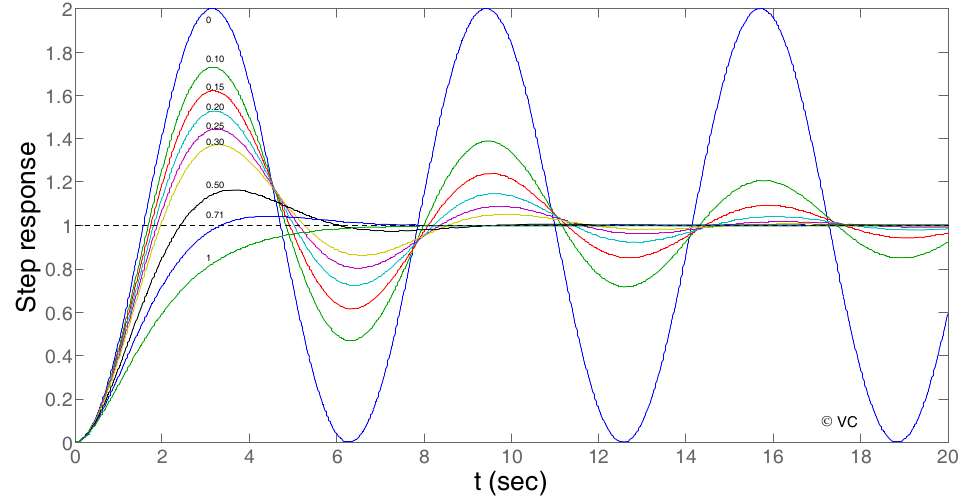
\includegraphics[width=0.6\textwidth]{risposta-al-gradino-unitario-di-un-sistema-del-secondo-ordine.png}
    \caption{Risposta Al Gradino Unitario Di Un Sistema Del Secondo Ordine}
    \label{fig:risposta-al-gradino-unitario-di-un-sistema-del-secondo-ordine}
\end{figure}
Posso ricavare che:
\[ \boxed{\hat{s} = e^{ -\frac{ \pi\zeta }{ \sqrt{1 - \zeta^{2}} } } } \]
\[ \boxed{ t_r = \frac{1}{\omega_n\sqrt{1-\zeta^{2}}} \cdot (\pi - \arccos(\zeta)) } \]
\[ \boxed{ t_{s,\alpha\%} = - \frac{\log(\alpha)}{\omega_n\zeta}  } \]
Questi sono idealmente i vincoli per $T$, nella realt\`a $T$ sar\`a diversa, anche se i vincoli risultanti da questo metodo saranno molto approssimati a quelli reali. Per diverse $T(s)$ mi servono:
\begin{itemize}
    \item \textbf{picco di risonanza} $T_p$:
        \[ T_p \triangleq \frac{\max\{|T(j\omega)|\}}{|T(j0)|}  \]
        \[ S_p \triangleq \max\{|S(j\omega)|\} \]
    \item \textbf{banda passante del sistema di controllo} $\omega _{BS}$:
        \[ \omega_{B}: |T(j\omega_{B})| = \frac{\sqrt{2}}{2} |T(j0)| \]
        \[ \omega _{BS}:  |S(j\omega_{BS})| = \frac{\sqrt{2}}{2} \text{ (non si usa) } \]
        Ovvero quando il modulo del guadagno diminuisce di $3dB$ (infatti $\frac{\sqrt{2}}{2} = -3dB$)
\end{itemize}
Il motivo per cui si studia anche la $S(s)$ \`e dato dal fatto che, alla fine dello studio del progetto, ci piacerebbe avere come risultato una funzione prototipo del secondo ordine, infatti se come risultato avessimo tale funzione $T_p$ e $S_p$ sarebbero equivalenti, ma cos\`i non sar\`a (nella maggior parte dei casi), per cui rafforziamo i nostri vincoli imponendoli anche su $S$ per fare in modo che, le specifiche del sistema siano quanto pi\`u vicine alle stesse specifiche di una funzione prototipo del secondo ordine.

Avendo una funzione prototipo del secondo tipo, la funzione ad anello pu\`o essere calcolata come:
\[ T(s): L(s) = \frac{T}{1 - T} \implies L(s) = \frac{\frac{\omega_n}{2\zeta} }{s \left( 1 + \frac{s}{2\zeta\omega_n}  \right) }  \]
La frequenza di crossover pu\`o essere espressa in funzione di $\zeta$ ed $\omega_n$:
\[ \boxed{ \omega_c = \omega_n \sqrt{\sqrt{1 + 4\zeta^{2}} - 2\zeta^{2}}  } \]
Possiamo allora esprimere il picco di risonanza e la banda in termini dei parametri:
\[ \boxed{T_p = \frac{1}{2\zeta\sqrt{1-\zeta^{2}}} } \]
\[ \boxed{S_p = \frac{2\zeta \sqrt{2 + 4\zeta^{2} + 2 \sqrt{1 + 8\zeta^{2}}}}{\sqrt{1 + 8\zeta^{2}} + 4\zeta^{2} - 1} } \]
\[ \boxed{\omega_B = \omega_n \sqrt{1 - 2\zeta^{2} + \sqrt{2 - 4\zeta^{2} + 4\zeta^{4}}}} \]


\begin{example}{}{}
    \[ \hat{s} \leqslant 10\%;\qquad t_r \leqslant 0.5s;\qquad t_{s,1\%} \leqslant 1.5s; \]
    Parto da $\hat{s}$, che dipende solo da un parametro:
\[ \hat{s} = e^{-\frac{\pi\zeta}{\sqrt{1 - \zeta^{2}}} } \implies \zeta = \frac{|\log(\hat{s})|}{\sqrt{\pi^{2} + \log^{2}(\hat{s})}} = 0.59 \implies \boxed{\zeta \geqslant  0.59 } \]
    Ricavo lo smorzamento, impongo $T_p$ ed $S_p$:
    \[ \boxed{T_p \leqslant \frac{1}{2\zeta\sqrt{1-\zeta^{2}}} \underset{\zeta = 0.59}{=} 1.05} \] 
    \[ \boxed{S_p \leqslant \frac{2\zeta \sqrt{2 + 4\zeta^{2} + 2 \sqrt{1 + 8\zeta^{2}}}}{\sqrt{1 + 8\zeta^{2}} + 4\zeta^{2} - 1} \underset{\zeta = 0.59}{=} 1.36} \]
    Consideriamo ora i requisiti sul tempo di salita:
    \[  t_r = \frac{1}{\omega_n\sqrt{1-\zeta^{2}}} \cdot (\pi - \arccos(\zeta))  \]
    \[   \omega_c = \omega_n \sqrt{\sqrt{1 + 4\zeta^{2}} - 2\zeta^{2}}  \]
    Otteniamo che:
    \[ t_r\omega_c =  \frac{1}{\sqrt{1-\zeta^{2}}} \cdot (\pi - \arccos(\zeta)) \cdot \sqrt{\sqrt{1 + 4\zeta^{2}} - 2\zeta^{2}} \]
    Quindi:
    \[ \boxed{\omega_c \geqslant \frac{1.97}{t_r} \underset{t_r = 0.5}{=} 3.94 rad/s} \]
    Similmente possiamo ottenere i requisiti per il tempo di settling:
    \[ t_{s,1\%} = \frac{4.61}{\omega_n\zeta}  \]
    Si ottiene:
    \[ t_{s,1\%}\omega_c \underset{\zeta = 0.59}{=} 5.64 \]
    Quindi:
    \[ \boxed{\omega_c \geqslant  \frac{5.64}{t_{s,1\%}} \underset{t_{s,1\%} = 1.5}{=} 3.76 rad/s} \]
    La traduzione delle specifiche porta a due valori delle frequnza di crossover diversi, per scegliere quella corretta si procede nel seguente modo:
    \[ \boxed{ \omega _{c,des} = \max\{ \underbrace{\omega_c}_{t_r}, \underbrace{\omega_c}_{t_{s,1\%}} \} \implies \omega_{c,des} = 3.94 rad/s } \]
\end{example}

\subsection{Luoghi di Magnitudo Costante}
Che valori deve assumere la $L(j\omega)$ per fare in modo che $|T(j\omega)|$ non superi mai $T _{p,max}$?

Per fare questa analisi,  usiamo una rappresentazine per il modulo di $T$.
\[ T = \frac{L}{1 + L} = \frac{u + jv}{1 + u + jv} = Me^{j\phi} \implies \begin{system} 
M^{2} = \frac{u^{2}+v^{2}}{(1 + u)^{2} + v^{2}} \\
\phi = \arctan\left( \frac{v}{u}  \right) - \arctan\left( \frac{v}{1+u}  \right) 
\end{system}  \]
Voglio trovare dei valori della parte reale e della parte immaginario di $L$ per cui $M^{2}$ ha gli stessi valori, dunque voglio trovare una formula per rappresentare un valore costante del modulo di $T$ al quadrato $M_T^{2}$. Facendo delle riscritture algebriche trovo che il luogo di punti che rispettano questa condizione sono:
\[ \implies \left( u - \frac{M_T^{2}}{1-M_T^{2}}  \right)^{2} +v^{2} = \left( \frac{M_T}{1-M_T^{2}}  \right)^{2}  \]
Questa rappresenta l'equazione di un cerchio:
\[ (u - C_u)^{2} + (v - C_v)^{2} = R^{2} \]
Infatti viene detto \textbf{cerchio $M_T$}:
\[ \implies M_T \text{ circle }: \begin{system}
    \displaystyle C  = \left( \frac{M_T^{2}}{1 - M_T^{2}}, 0 \right) & \text{,(centro)} \\
    \\
    \displaystyle R = \left| \frac{M_T}{1 - M_T^{2}}  \right|  & \text{,(raggio)}
\end{system}  \]
\begin{figure}[H]
    \centering
    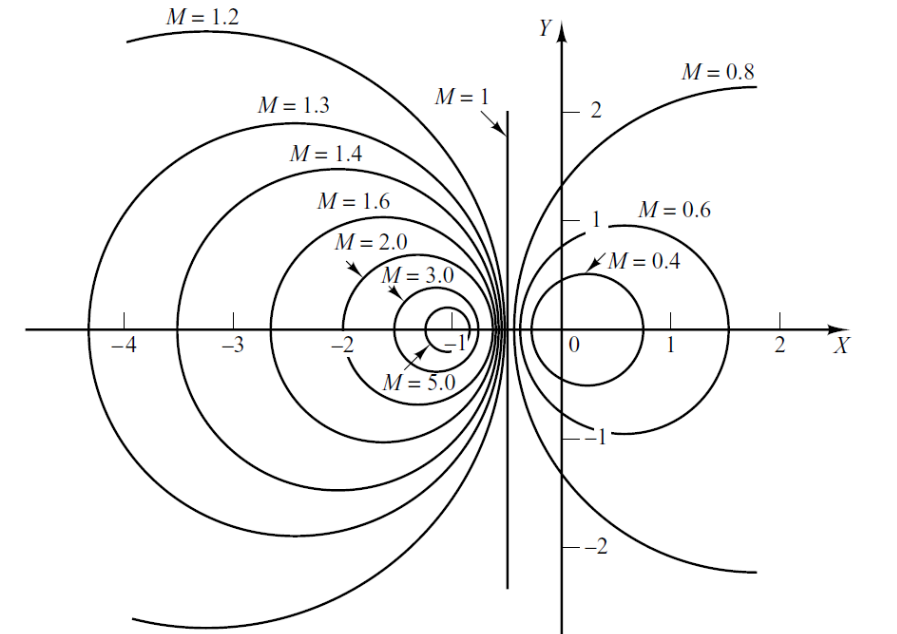
\includegraphics[width=0.6\textwidth]{luogo-dei-punti-del-cerchio-mt.png}
    \caption{Luogo Dei Punti Del Cerchio Mt}
    \label{fig:luogo-dei-punti-del-cerchio-mt}
\end{figure}
Supponiamo quindi di avere un vincolo sulla massima sovraelongazione, ad esempio $T_p \leqslant 6$. Non deve mai accadere che il Diagramma Polare della funzione ad anello attraversi la regione contenuta all'interno del cerchio di raggio $M_T = 6$, ci\`o significherebbe che il valore di $T_p$ viene superato da $|T(j\omega)|$ e ci\`o non deve accadere. Plottando queste condizioni, si possono modificare apportunamente gli zeri i poli della funzione ad anello per far si che vengano rispettati i vincoli, per far ci\`o si usano i Diagrammi di Nichols, che rendono pi\`u comoda la visualizzazione della funzione, dove le regioni formate dai cerchi verranno deformate come delle ellissi.



\begin{problem}{}{}
    4. $|e _{d_p}^{\infty}| \leqslant 5\cdot 10^{-4}$, $d_p(t) = a_p\cdot \sin(\omega_p t), |a_p| \leqslant 2\cdot 10^{-2}, \omega_p \leqslant 0.02 rad/s$.
    \[ |e _{d_p}^{\infty}| = |y^{\infty} _{d_p}| = |a_p |G(j\omega_p)| \sin(\omega_p t + \phi)| \leqslant |a_p| |G(j\omega_p)| \]

    ...

5. $e _{d_s}^{\infty}$

% TODO:  <24-05-22, da finire> %
\end{problem}



\subsection{Scelta di Kc}
Quando si \`e trovato il modulo di $K_c$ minimo si prende un valore leggermente pi\`u grande dei requisiti minimi. Per \textbf{scegliere il segno del modulo di $K_c$}, e quindi di garantire la stabilit\`a, \`e necessario vedere il numero di encircolamenti di $L$ intorno a $-1+j0$, assegnamo un valore arbitrario tra positivo e negativo, se $P_{cl}$ \`e un numero pari allora il segno va bene, altrimenti il segno va invertito. 

\subsection{Progetto di LEAD e LAG}
Ogni rete \`e un filtro del primo ordine, come si vede in (\ref{def:controllore}). Per progettare questa rete si usa un metodo detto \textbf{loop-shaping design}.

Per garantire le specifiche del transitorio, si deve garantire che, inserendo le reti LEAD e LAG, il Diagramma di Nichols di $L$ non entri all'interno delle regioni proibite, anche se questa condizione non \`e necessario n\'e sufficente a garantire le specifiche sulla sovraelongazione, qusto \`e dato dal fatto che la $T$, in generale, non \`e equivalente alla funzione prototipo, dunque il suo comportamento si discosta leggermente da quello che ci aspettiamo, ci\`o nonostante, rispettare le zone \`e comunque un buon indicatore per il rispetto delle specifiche. Stare al di fuori delle regioni proibite garantisce un livello di robustezza: il progetto del controllore comporta degli errori, dati dalla differenza tra modello matematico e quella che \`e la realt\`a, sono presenti anche errori dati dalla linearizzazione, allora la funzione ad anello nella realt\`a sar\`a diversa da quella trovata, e se si trova vicino al punto ciritico ($-1 + j0$), data la presenza di errori, si rischia di attraversarlo. Uscendo dalle regioni proibite spostiamo la fase ed il modulo lontano dal punto critico (in molti libri di testo vengono definite delle distanze dette \textbf{margine di fase } e \textbf{margine di guadagno}, per garantire la robustazza, ma questo non garantisce che  in un intorno non ci si possa avicinare al punto critico, \`e anche per questo motivo che si usano le regioni proibite).

\textbf{Criteri per scegliere la frequenza di cross-over desiderata} (durante l'esame la scelta va motivata):
\begin{itemize}
    \item se la prendo vicino al limite superiore, si ha il comportamento pi\`u veloce per il transitorio;
    \item se la prendo vicino al limite inferiore, si ottiene un attenuzazione maggiore dei disturbi;
\end{itemize}


Guardo l'intervallo e scelgo una $\omega _{c,des}$ e vado a vedere dove viene mappato il punto sul diagramma di Nichols. Quel punto, essendo la frequenza di crossover, deve avere un guadagno di $0dB$. Per fare questo potrei semplicemente aumentare il guadagno e quindi traslare il grafico in alto, ma in contemporanea devo traslare anche orizzontalmente, altrimeti si rischia di far diventare instabile il sistema. Per fare ci\`o si pu\`o semplicemente aggiungere uno zero al controllore, ma ogni volta che si aggiunge uno zero, si deve anche aggiungere un polo, questo \`e dovuto al fatto che il controllore deve sempre essere realizzabile, dunque il grado del numeratore deve sempre essere minore o uguale al grado del denominatore, il polo che si aggiunge cacella la fase che viene aggiunta dallo zero. Per evitare che il contributo venga completamente annullato nell'intorno in cui si vuole applicare lo zero, il polo avr\`a una fase maggiore dello zero, il comportamento di tale \`e detto di \textbf{compana di fase}, che avr\`a un'effetto di diminuire il gudagno e di aumentare la fase alla frequenza di crossover.
\begin{figure}[H]
    \centering
    \subfloat[Rete LEAD Su Nichols]{%
        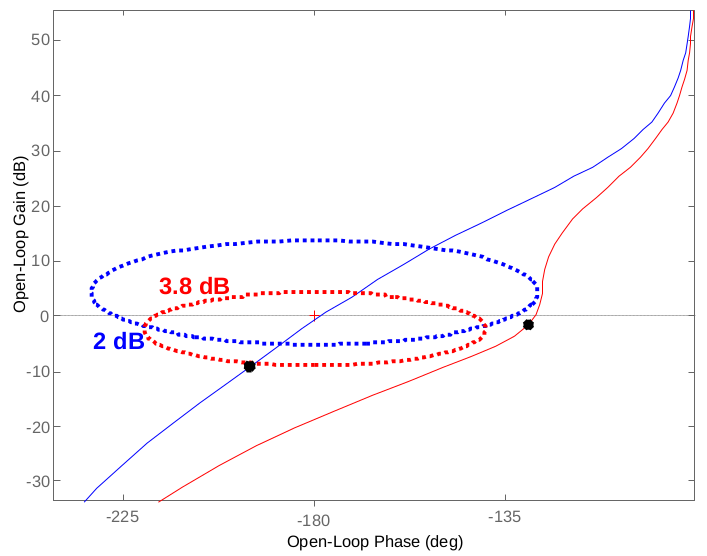
\includegraphics[width=0.4\textwidth]{rete-LEAD-su-nichols.png}%
        \label{rete-LEAD-su-nichols}%
        }%
    \hfill%
    \subfloat[Bode Rete LEAD]{%
        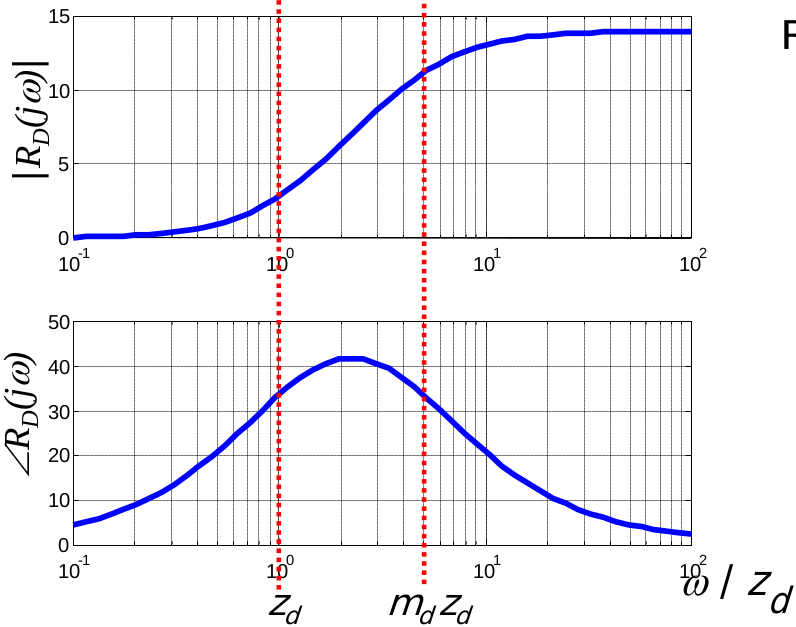
\includegraphics[width=0.4\textwidth]{guadagno-e-fase-rete-LEAD.png}%
        \label{guadagno-e-fase-rete-LEAD}%
        }%
    \caption{Effetto rete LEAD}
\end{figure}

\[ R_d(s) = \frac{\displaystyle 1 + \frac{s}{z_d} }{\displaystyle 1 + \frac{s}{m_dz_d} }\;,\quad m_d > 1  \]
\begin{itemize}
    \item $m_d$ determina quanto sar\`a grande la compana di fase;
    \item $z_d$ detemina in frequenza dove sar\`a posizionata la compana di fase.
\end{itemize}

Si pu\`o mostrare che partendo una fuznione prototipo del secondo ordine $T_2$, e ricavando $L_2$ da essa, il diagramma di Nichols di $L_2$ passa tangente a entrambe le regioni proibite. Quello che vorremmo ottenere \`e che:
\[ T \simeq T_2 \implies L \simeq L_2 \]
Se definisce una fascia di valori in cui si vuole che il comportamento della funzione ad anello ricavata sia simile a quello della funzione prototipo.

% TODO:  <25-05-22, mettere figure delle T che si approssima a T_2> %


Consideriamo una situazione differente, per introdurre la rete LAG. Ad esemio la mia $\omega _{c,des}$ si trova al di sopra dei $0dB$, per fare in modo di abbassare il suo modulo si inserisce un modulo nel controllore. Inserendo un polo, qeusto va a deteriorare la fase, che mi comporta nella maggior parte dei casi un attraversamento della zona proibita, aggiungendo uno zero a fase maggiore del polo si reisce avere un comportamento sulla fase simila quello precdente in un introrno della frequnza a cui si \`e diminuito il modulo.
\begin{figure}[H]
    \centering
    \subfloat[Rete LAG Su Nichols]{%
        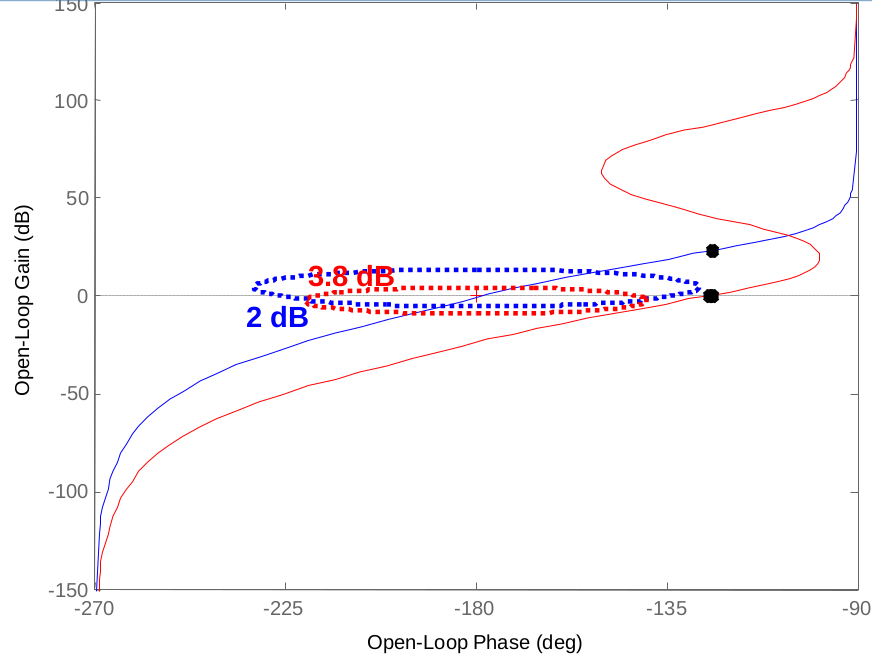
\includegraphics[width=0.4\textwidth]{rete-LAG-su-nichols.png}%
        \label{rete-LAG-su-nichols}%
        }%
    \hfill%
    \subfloat[Bode Rete LAG]{%
        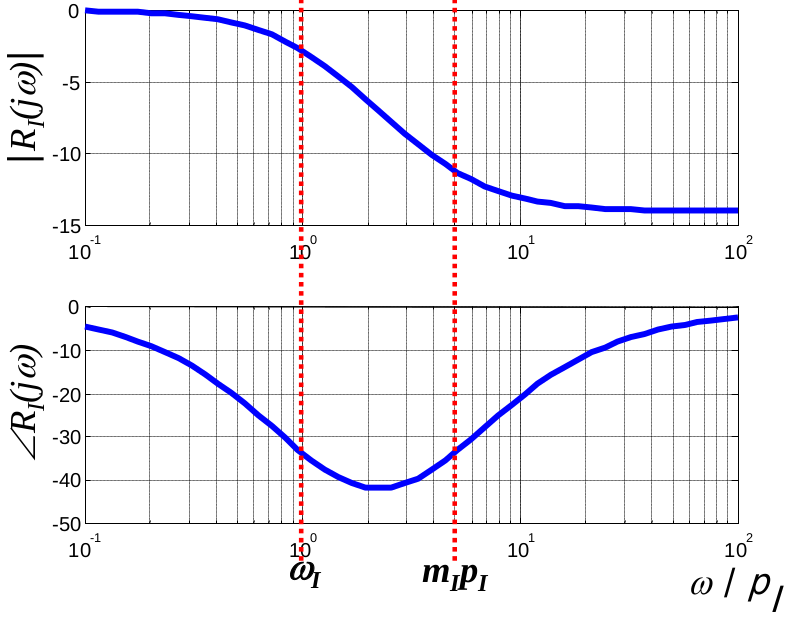
\includegraphics[width=0.4\textwidth]{bode-rete-LAG.png}%
        \label{bode-rete-LAG}%
        }%
    \caption{Effetto rete LAG}
\end{figure}

\[ R_i(s) = \frac{\displaystyle 1 + \frac{s}{m_ip_i} }{\displaystyle 1 + \frac{s}{p_i} }\;,\quad m_i > 1  \]

Considerazioni:
\begin{itemize}
    \item Non ci sono effetti negativi nell'introduzione di una rete LEAD;
    \item Progettando una rete LAG si vuole ottenere solo uno dei due effetti che provoca, ovvere un abbassamento del modulo senza la perdita di fase, che \`e indesiderata, inoltre, una consegunza provocata dall'inserimento dalle reti LAG \`e l'\textbf{effetto coda};
\end{itemize}

...


Rete derivativa: prendo la differenza tra la fase alla frequenza di $\omega_{c,des}$ e la fase che si trova al di fuori delle regioni proibite.

Quindi trovo la 

"Progetto una rete LEAD con $\omega$ normalizzata = 1.2 e m = .. al fine di recuperare $\deg{45}$ all $\omega_{c,des} = 0.8 rad/s$",

La $\omega_{norm} \triangleq \frac{\omega _{c,des}}{z_d} \iff 1.2 = \frac{0.8}{z_d}$


Per la reta LAG si prende sempre un valore della $\omega _{norm}$ di 100
Il modula deve scendere di (pu\`o essere calcolato analiticamente):
\[ \lim_{s \to \infty} R_i(s) = \lim_{s \to \infty} \frac{1 + \frac{s}{m_ip_i} }{1 + \frac{s}{p_i} } = \frac{p_i}{m_ip_i} = \frac{1}{m_i}   \]

...

Valuto le prestazioni del sistema, valutando con una prestazione che tutte esse siano verificate.

...

Le reti LAG causano l'\textbf{effetto coda}: progettando una rete di tipo LAG, andiamo a inserire una frequenza normalizzata che diventer\`a uguale alla frequnza di crossover. Utilizzando la rete LAG, avr\`o uno zero ed un polo a bassa frequnza. La funzione $T$ \`e uguale a $\frac{L}{1 + L}$, questo comporta che gli zeri di $T$ sono coincidenti con gli zeri di $L$, questo implica che gli zeri del controllore sono zeri di $T$. Ma deve rimanere vero il fatto che $T$, a bassa frequenza deve essere 1, dunque vicino allo zero, per forza di cose, deve comparire un polo (dato da $1 + L$ al denominatore), si pu\`o provare che il residuo di quel polo \`e motlo basso, quindi avremmo un'esponenziale in uscita che decresce lentamente (dato dal fatto che il polo si trova a bassa frequenza), ed ha un ampiezza molto ridotta, questo effetto non si nota perch\`e il modello utilizzato per la $T$ era quello di una fuznione prototipo del secondo tipo, nella quela non era presente nessun polo a basso frequenza. Questo problema non si pone nelle reti LEAD, perch\`e il polo si trova ad alta frequenza, perch\`e gli eventuali esponenziali decrescono molto velocemente ed il modulo di $T$ scnende molto velocemnte.

Esiste un altro tipo di rete derivativa, detta \textbf{rete zero}, composta da un singolo zero. Questa rete \`e utilizzabile solo nul caso in cui $\nu$ sia maggiore di 0, infatti \`e possbile usare un numero $\nu$ di volte reti di tipo zero. La rete zero \`e la rete pi\`u raccomandata da utilizzare, nel caso in cui sia possibile farlo.



\newpage
\section{Sistemi a Tempo Discreto}

...

Il sistema \`e stabile quando valgono le condizini: $|\lambda_i| < 1,\; \forall i$

\begin{definition}{D Stabilit\`a BIBO}{d-stabilita-bibo}
    Un sistema \`e BIBO stabile se e solo tutti i poli della \emph{f.d.t.} hanno modulo strettamente minore di 1.
\end{definition}

La definizione del punto di equilibro \`e molto simile a quello a tempo continuo. Per valere la condizione di stabilit\`a deve valere che:
\[ \boxed{x(k+1) = x(k)} \]
Questo \`e dato dal fatto che in tempo discreto non esiste la derivata.
Dunque per imporre il punto di equilibrio:
\[ \begin{system} 
\vv{f}(\bar{\vv{x}}, \bar{\vv{u}}) = \bar{\vv{x}} \\
\vv{g}(\bar{\vv{x}}, \bar{\vv{u}}) = \bar{\vv{y}}
\end{system}  \]
Anche in questo caso, trovato il punto di equilibrio di un sistema, si pu\`o linearizzare il sistema, attraverso l'uso delle matrici Jacobiane.






% TODO:  <15-05-22, rifare la parte sui diagrammi che fa schifo> %



\newpage
\section{Problemi d'Esame}
Qua verranno svolti i passaggi su matlab di esempi di temi di esame.

\subsection{Problema 1}
hmm





\end{document}
